\documentclass[11pt]{article}
\usepackage[utf8]{inputenc}
\usepackage{graphicx}
\usepackage{graphics}
\usepackage{lipsum}
\usepackage{caption}
\usepackage{subcaption}
\usepackage[a4paper,width=150mm,top=30mm,bottom=30mm]{geometry}
%\usepackage{minted}
\usepackage{hyperref}
\usepackage{fancyhdr}
\usepackage{float}
\pagestyle{fancy}
\fancyhead{}
%\fancyhead[R]{Text}    % add text as header
\fancyfoot{}
\fancyfoot[C]{\thepage}   % add page number
\renewcommand{\headrulewidth}{0.10pt}
\renewcommand{\footrulewidth}{0.10pt}

%% \pagestyle{empty} remove header and footer for that page
%% \pagestyle{plain} add only the page number

\usepackage[
    backend=biber, 
    natbib=true,
    sorting=none
]{biblatex}
\addbibresource{references.bib}

\begin{document}



\begin{titlepage}
    \begin{center}
        \vspace*{1cm}
        
        \Huge
        \textbf{Computational Human Genomics Project}

        \vspace{0.3cm}

        \rule{\textwidth}{.4pt}

        \vspace{0.5cm}
        
        \LARGE
        Variant Calling and Annotation, Ancestry analysis, Tumor Ploidy and Purity assessment.
        
        
        \vfill

        \Large
        
        \textbf{Linda Cova and Enrico Frigoli}
        
        \vspace{1cm}
        
        Github: \href{https://github.com/enricofrigoli/chg\_project.git}{https://github.com/enricofrigoli/chg\_project.git}
        
        \vspace{0.8cm}
        
        %\includegraphics[width=0.4\textwidth]{logo}
        
        \Large
        Computational Human Genomics  \\
        Prof. Demichelis, Prof. Romanel \\
        University of Trento \\
        A.Y. 2021-2022

        
    \end{center}

\end{titlepage}

%\twocolumn[
%  \begin{@twocolumnfalse}
%    \begin{abstract}
%        \centering
%        Cancer genomics is the coolest thing in the world.
%    \end{abstract}
%  \end{@twocolumnfalse}
%]

% \parencite{}

%\vspace*{1cm}



\section*{Introduction}

The study of somatic and germline variations (SNPs, SNVs, indels, CNVs and SVs) is of key importance in the field of cancer genomics, as these lead to altered gene function in cancer. Although many tools and pipelines have been developed in recent years to tackle the problem, these variations are still challenging to identify. Here, we describe the use of different tools to analyse germline variants, somatic variants, ancestry, tumor ploidy and purity, and to perform additional analysis on provided data. 




\section*{Methods}

To perform the required analysis, two setups were used: the first one (hereafter setup \textbf{1}) involves the use of a provided Virtual Machine that already included GATK (v3.8-1-0), Picard (v2.22.3), VarScan (v2.3.9), and snpEff (v4.3t); since some of the included tools are no longer considered best-practice and variant calling works better by combining different tools, a second setup was used (hereafter setup \textbf{2}), consisting of GATK (v4.2.6.1) run in a Docker container with Picard (v2.27.1), and SnpEff (5.1d). Both setups share custom R scripts, the provided raw BAM files, few files containing the reference genome, the .bed files containing the captured regions and the .vcf files for variant annotation. The code with additional details can be found on \href{https://github.com/enricofrigoli/chg_project.git}{github}. The two provided BAM files contain already selected fractions of data from a breast cancer sample and matched control from TCGA (TCGA-A7-A4SE).


\subsection*{Data inspection}

Each of the two BAM files can be inspected either using \texttt{samtools stats [filename]} or \texttt{samtools flagstat [filename]}, for detailed and general statistics respectively. 


\subsection*{Preprocessing of BAM files}

In order to be used for subsequent analysis, BAM files containing raw mapped reads must undergo several preprocessing steps; however, different variant calling tools require different preprocessing procedure. A common first step is deduplication: this allows to remove technical duplicates among the pool of reads that could bias the discovery of variants. 
After sorting and indexing with \texttt{samtools}, deduplication was performed with \texttt{MarkDuplicates} tool of Picard, using as additional parameters \texttt{-ASSUME\_SORT\_ORDER coordinate}, \texttt{ -M Control\_dedup\_metrics.txt} and \texttt{-REMOVE\_DUPLICATES true}.

Common steps after duplicates removal are realignment and recalibration; while recalibration is always needed before performing downstream analysis, different tools may require or not realignment. Here, realignment was performed with \texttt{RealignerTargetCreator} and \texttt{IndelRealigner} (setup 1) specifying as parameter the reference genome and the .bed files containing the captured regions.
The number of realigned reads was retrieved with \texttt{grep "OC" | wc -l} piped from the output of \texttt{samtools view [filename]}.
Recalibration was performed on the realigned files with \texttt{BaseRecalibrator} and \texttt{PrintReads} (setup 1), and on the raw files with \texttt{BaseRecalibrator} and \texttt{ApplyBQSR} (setup 2). In both cases the results of the recalibration were plotted using \texttt{AnalyzeCovariates}, together with a second recalibration on already recalibrated files that was run as a quality control.
The number of recalibrated reads can be retrieved with \texttt{samtools view [filename] | grep "OQ" | wc -l}, where "OQ" stands for \emph{Original Quality}, that was set to be emitted during recalibration using the parameter \texttt{--emit-original-quals}.



\subsection*{Germline Variant Calling}

Germline variants (SNPs and indels) were called differently based on the setup in use. With the setup 1, variants were called with \texttt{UnifiedGenotyper} using, as additional input, the reference genome and the .bed file containing the captured regions. SNPs calls were filtered and selected (omitting indels) with \texttt{vcftools}, using the following input: \texttt{--minQ 20 --max-meanDP 200 --min-meanDP 5} to filter variants with min quality of 20, max depth across samples of 200 and min of 5, \texttt{--remove-indels --recode --recode-INFO-all} to remove indels, output the filtered vcf and keep all INFO variables respectively. 

Since \texttt{UnifiedGenotyper} is now considered a legacy tool, a more updated one was also used. For this purpose, we decided to use \texttt{HaplotypeCaller} (setup 2) following the pipeline recommended by GATK for small germline variant discovery (Figure \ref{pipeline_germline_variant}), that recommends to call variants without a realignment step; this is the case since the tool also performs a sort of assembly in active regions, removing the need of upstream realignment. Following GATK recommendation, the raw callset was filtered with \texttt{CNNScoreVariants}, that annotates the obtained VCF with scores generated from a CNN (Convolutional Neural Network) using a 2D model with pre-trained architecture, indicating the model's prediction of the quality of each variant, based on the genomic context. Indels were then removed to keep only SNPs using \texttt{SelectVariants} with \texttt{--select-type-to-include SNP} as parameter. The callset was further refined using \texttt{FilterVariantTranches}, that filters variants based on the score assigned by \texttt{CNNScoreVariants} using as additional resource the \texttt{hapmap\_3.3.b37.vcf} file.

In both cases the number of heterozygous SNPs was calculated with basic bash commands: \texttt{cat [filename.vcf] | grep "0/1" | wc -l}, as "0/1" is the annotation of heterozygous SNPs in VCF files. The vcf file containing only heterozygous SNPs was retrieved using \texttt{grep -E "(\^\ \#|0/1)"}.
The intersection between the two callsets was computed with \texttt{bedtools intersect} and \texttt{vcftools --diff-site}, to see what was the concordance between the two different variant caller.

The refined callsets were annotated with \texttt{SnpEff}\cite{cingolani2012program} and its submodule \texttt{SnpSift}\cite{cingolani2012using}, using the \texttt{hapmap\_3.3.b37.vcf} file and \texttt{clinvar\_Pathogenic.vcf}. SnpSift \texttt{filter} function was also used to select clinically significant variants annotated in Clinvar with the following expression \texttt{"(exists CLNSIG)"}. 



\subsection*{Somatic Variant Calling}

As it was done for germline small variants, also somatic ones were called using two different tools: VarScan2 and Mutect2. 

To perform somatic point mutations calling with the setup 1, both Control and Tumor files were given as input to \texttt{samtools mpileup}, along with the reference genome, to compute the pileups, which were then used to call variants with \texttt{VarScan somatic} using \texttt{--output-snp somatic.pm --output-vcf 1} as parameters to select for SNPs and produce a .vcf file. The callset at this point included also germline variants, so only somatic ones were filtered using \texttt{grep}. The filtered callset was then annotated with SnpEff specifying \texttt{hg19} as internal dataset to be used.

The setup 2 instead involved the use of Mutect2 (from GATK): as parameters were given the BAM files, the bed file containing captured regions, the reference genome, and the filtered callset of germline variants found with \texttt{HaplotypeCaller} (setup 2). The callset was filtered using \texttt{FilterMutectCalls} and annotated with snpEff using again the internal hg19 dataset (the use of \texttt{Funcotator} is recommended but its complexity places it beyond the purposes of this analysis). 

Somatic CNVs were called with VarScan (setup 1) running the \texttt{copyCaller} command on pileups file; the resulting output was processed in R using the package \texttt{DNAcopy} (version 1.68.0) \cite{DNAcopy}. A circular binary segmentation was performed to point out regions with copy-number aberrations with the following parameters: 2 as minimum number of markers in a segment, 3 as minimum standard deviation between splits, \textit{alpha}=0.05 as the significance threshold to distinguish two segments and 100 as the number of permutations used to compute the P-value.


\subsection*{Variants in DNA Repair Genes}

The identification of SCNAs overlapping with DNA repair genes was performed in R: the segments containing DNA repair genes were individuated and their mean log2 ratio was analysed to identify copy-number aberrations. With the same purpose, starting from the bed file containing heterozygous deletions and intersecting it with the file \texttt{DNA\_Repair\_Genes.bed}, another .bed file was retrieved containing DNA repair genes that were subject to somatic heterozygous deletions. Another intersection was performed between the callset of heterozygous pathogenic SNPs (containing only the one in \emph{BRCA1}) and the new bed file, using again \texttt{bedtools intersect}. 

Since only one variant was pathogenic, another intersection was perfomed between the .bed file previously obtained and the entire callset of heterozygous SNPs found with \texttt{HaplotypeCaller} (setup 2). This allowed to retrieve also other germline SNPs that were not annotated as pathogenic but still residing into fragments that later underwent somatic heterozygous deletions (found in the Tumor sample). 

The same approach was also used to see whether called somatic small variants (point mutations and indels) were present in the subset of DNA repair genes harboring somatic heterozygous deletions. For this purpose, the callset generated with Mutect2 (setup 2) was used, since Varscan (setup 1) identified far less somatic variants.
The output of the intersection between the callset and \texttt{DNA\_Repair\_Genes.bed} was formatted in bash and used as input to a custom R script that allowed to intersect the list of DNA repair genes with the one of heterozygous deletions (as could have been done with \texttt{bedtools intersect}) to generate a plot to show the number of somatic variants (point mutations and indels) for each DNA repair gene harboring a somatic heterozygous deletion.



\subsection*{Ancestry Analysis}

The ancestry analysis was performed with the R package \texttt{EthSEQ}\cite{ethseq}. The control sample preprocessed (setup 1) BAM file was provided as target input. The reference model was provided in gds format with the \texttt{SS2.Light.Model.gds} file. The function \texttt{ethseq.Analysis} relies on the \texttt{ASEQ} R package to genotype the BAM file on positions indicated by the reference model and creates a target model. Only SNPs that satisfy the requirements given as parameters are retained (minimum base quality = 20, minimum read quality = 1, minimum read count =10) and a PCA is performed on the aggregated target and reference models. For each ethnicity, an area is individuated in the 3D space and the sample is classified based on where its principal components fall in this space.


\subsection*{Purity and Ploidy estimation}

Tumor purity was inferred with the R packages \texttt{CLONETv2} (version 2.2.1)\cite{clonet} and \texttt{TPES} (version 1.0.0)\cite{tpes}, that rely respectively on somatic copy-number changes and somatic point mutations.

Read counts per allele were computed with the \texttt{ASEReadCounter} tool (GATK) on the processed control and tumor BAM files (setup 1) considering the SNP sites individuated in the "germline variant calling" section. These were coupled with the segmentation data in order to retrieve the \textit{beta} table, following the \texttt{CLONETv2} workflow. The beta values are the percentages of neutral reads per segment and are useful to infer tumor ploidy, which in turn is computed considering the log ratio between tumor and control coverage within each segment LogR, normalized over the ratio between the mean tumor and control coverage. With the ploidy and beta tables it is possible to calculate the admixture: the percentage of non-tumor cells in a tumor sample, equivalent to 1-purity. The standard parameters were maintained for all the \texttt{CLONETv2} functions.

On the other hand, the \texttt{TPES} workflow requires as input the SNVs identified in the "somatic variant calling" section with VarScan, in addition to the ploidy and segmentation data. This tool selects copy-number neutral segments, and, after applying a threshold on allelic fraction (maxAF=0.55) and reference mapping bias (RMB=0.47), identifies putative clonal SNVs and exploits them to assess tumor purity.


\subsection*{SPIA test}

Read counts per allele were obtained with \texttt{ASEReadCounter} (GATK), giving as input the preprocessed (setup 1) BAM files for the tumor and control samples and considering all the SNP sites provided by the \texttt{hapmap\_3.3.b37.vcf} file. The SPIA test is an assay aimed at the individuation of different cell lines, usually employed to discriminate between samples from different patients or to confirm that multiple samples have the same origin. The test was performed with the R package \texttt{SPIAssay} (version 1.1.0)\cite{spia}, which uses the genotype of the provided SNPs (classified as homozygous reference, homozygous alternative or heterozygous) of both samples to compute a distance score and assigns a SPIA score that classifies the two samples as \textit{similar}, \textit{different} or \textit{uncertain}.





\section*{Results}

\paragraph{Data inspection and pre-processing}
The number of properly paired reads was retrieved from the statistics generated for the two BAM files (\texttt{Control.bam} and \texttt{Tumor.bam}), and were 19576046 (99.33\%) and 14979936 (99.67\%) respectively. 
After realignment, the number of realigned reads (setup 1) was 2445 for the Control file and 1937 for the Tumor file. 

The results of the recalibration steps are summarized in the plots (Figures \ref{recal_control_1}-\ref{recal_tumor_2}); the process resulted in higher quality score accuracy and slightly lower mean quality score. As expected, recalibration worked better on realigned BAM files, since artifactual SNPs are replaced with real indels (recalibration for the setup 2 not shown). Although successful, recalibration plots usually show better results with increasing size of input data: since this analysis was performed on small data, a higher noise in recalibration plots is expected. 

\paragraph{Germline variant calling} 
Since two germline variants caller were used, it was possible to compare the resulting callsets: the filtered one obtained with \texttt{UnifiedGenotyper} contained 6480 heterozygous SNPs, while the filtered one obtained with \texttt{HaplotypeCaller} contained 6937 heterozygous SNPs; 5933 of them were common between the two files. 

When looking for pathogenic variants (which is by definition a variant that is well characterized and strongly associated with a high increase in the risk of developing a pathology), both callers identified only the variant in BRCA1 gene, associated with hereditary breast and ovarian cancer syndrome (Figure \ref{igv_BRCA1}). This is indeed the type of cancer from which the tumor sample was retrieved.

\begin{figure}[H]
   \centering
   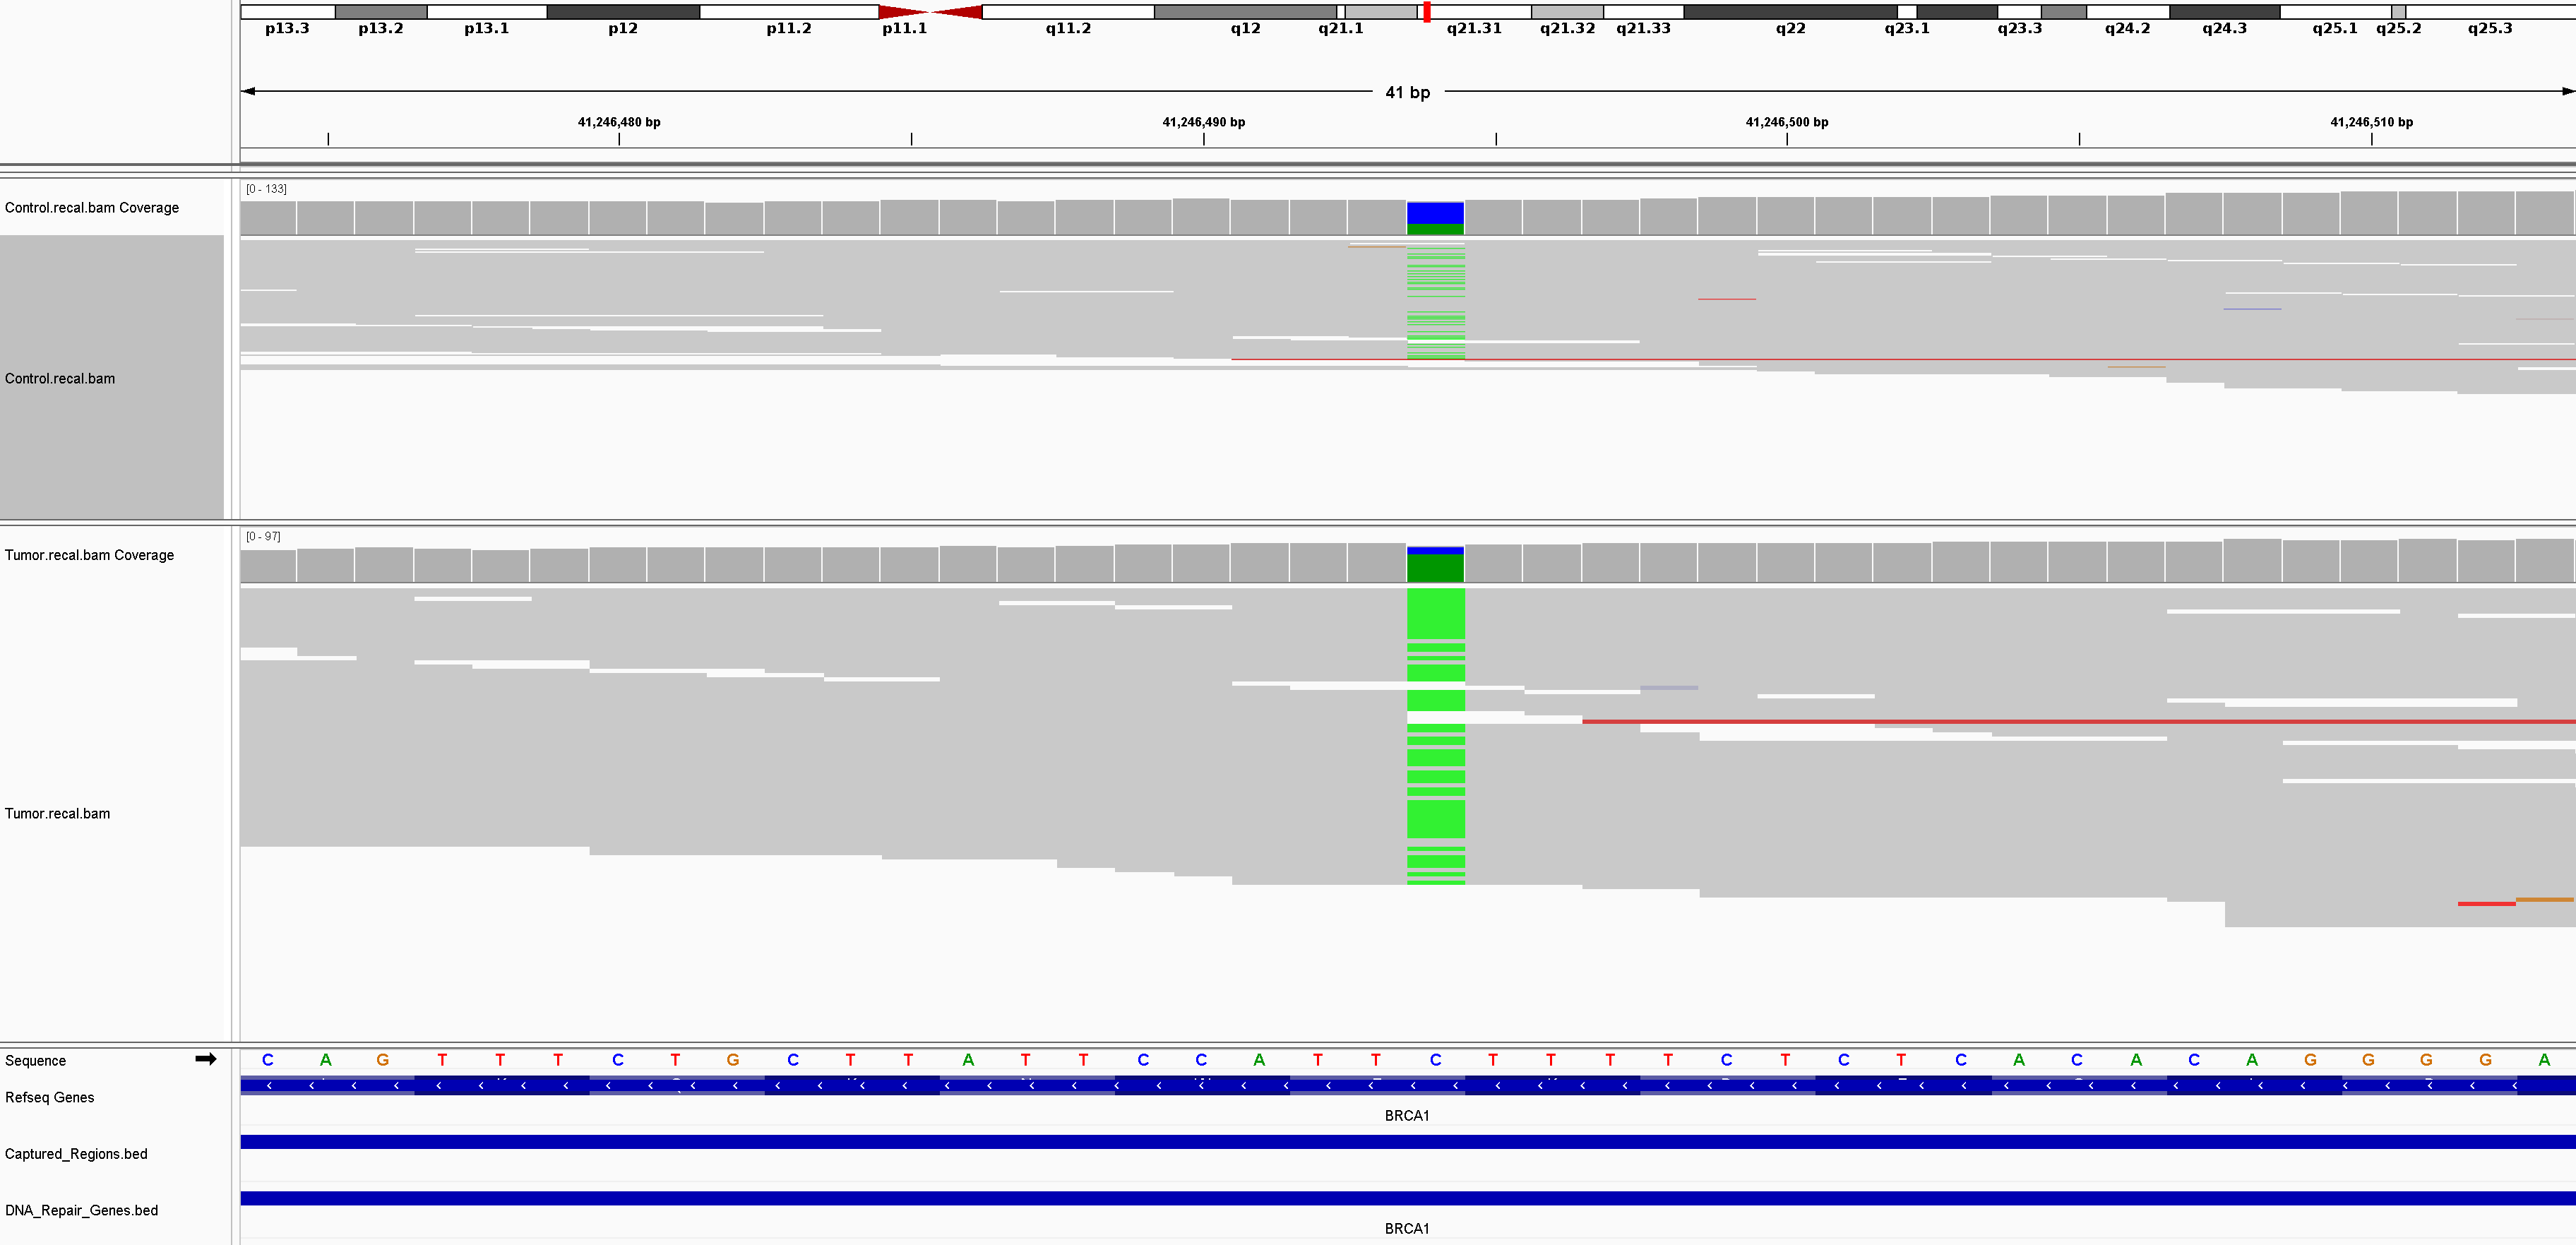
\includegraphics[width=\textwidth]{images/BRCA1_snp_het_del.png}
   \caption{\footnotesize{Snapshot from IGV on the SNP in BRCA1 associated with hereditary breast and ovarian cancer at position chr17:41246494; see Results section for the biological implication of the change in the allelic fraction of the alternative base.}}
   \label{igv_BRCA1}
\end{figure}


\paragraph{Ancestry analysis}
The ancestry analysis determined that the patient is of African ethnicity. The first three principal components (respectively: 0.053, 0.003 and -0.003) place the control sample perfectly into the 3D space associated with the African population (Figure \ref{ethSEQ}).

\begin{figure}[H]
   \centering
   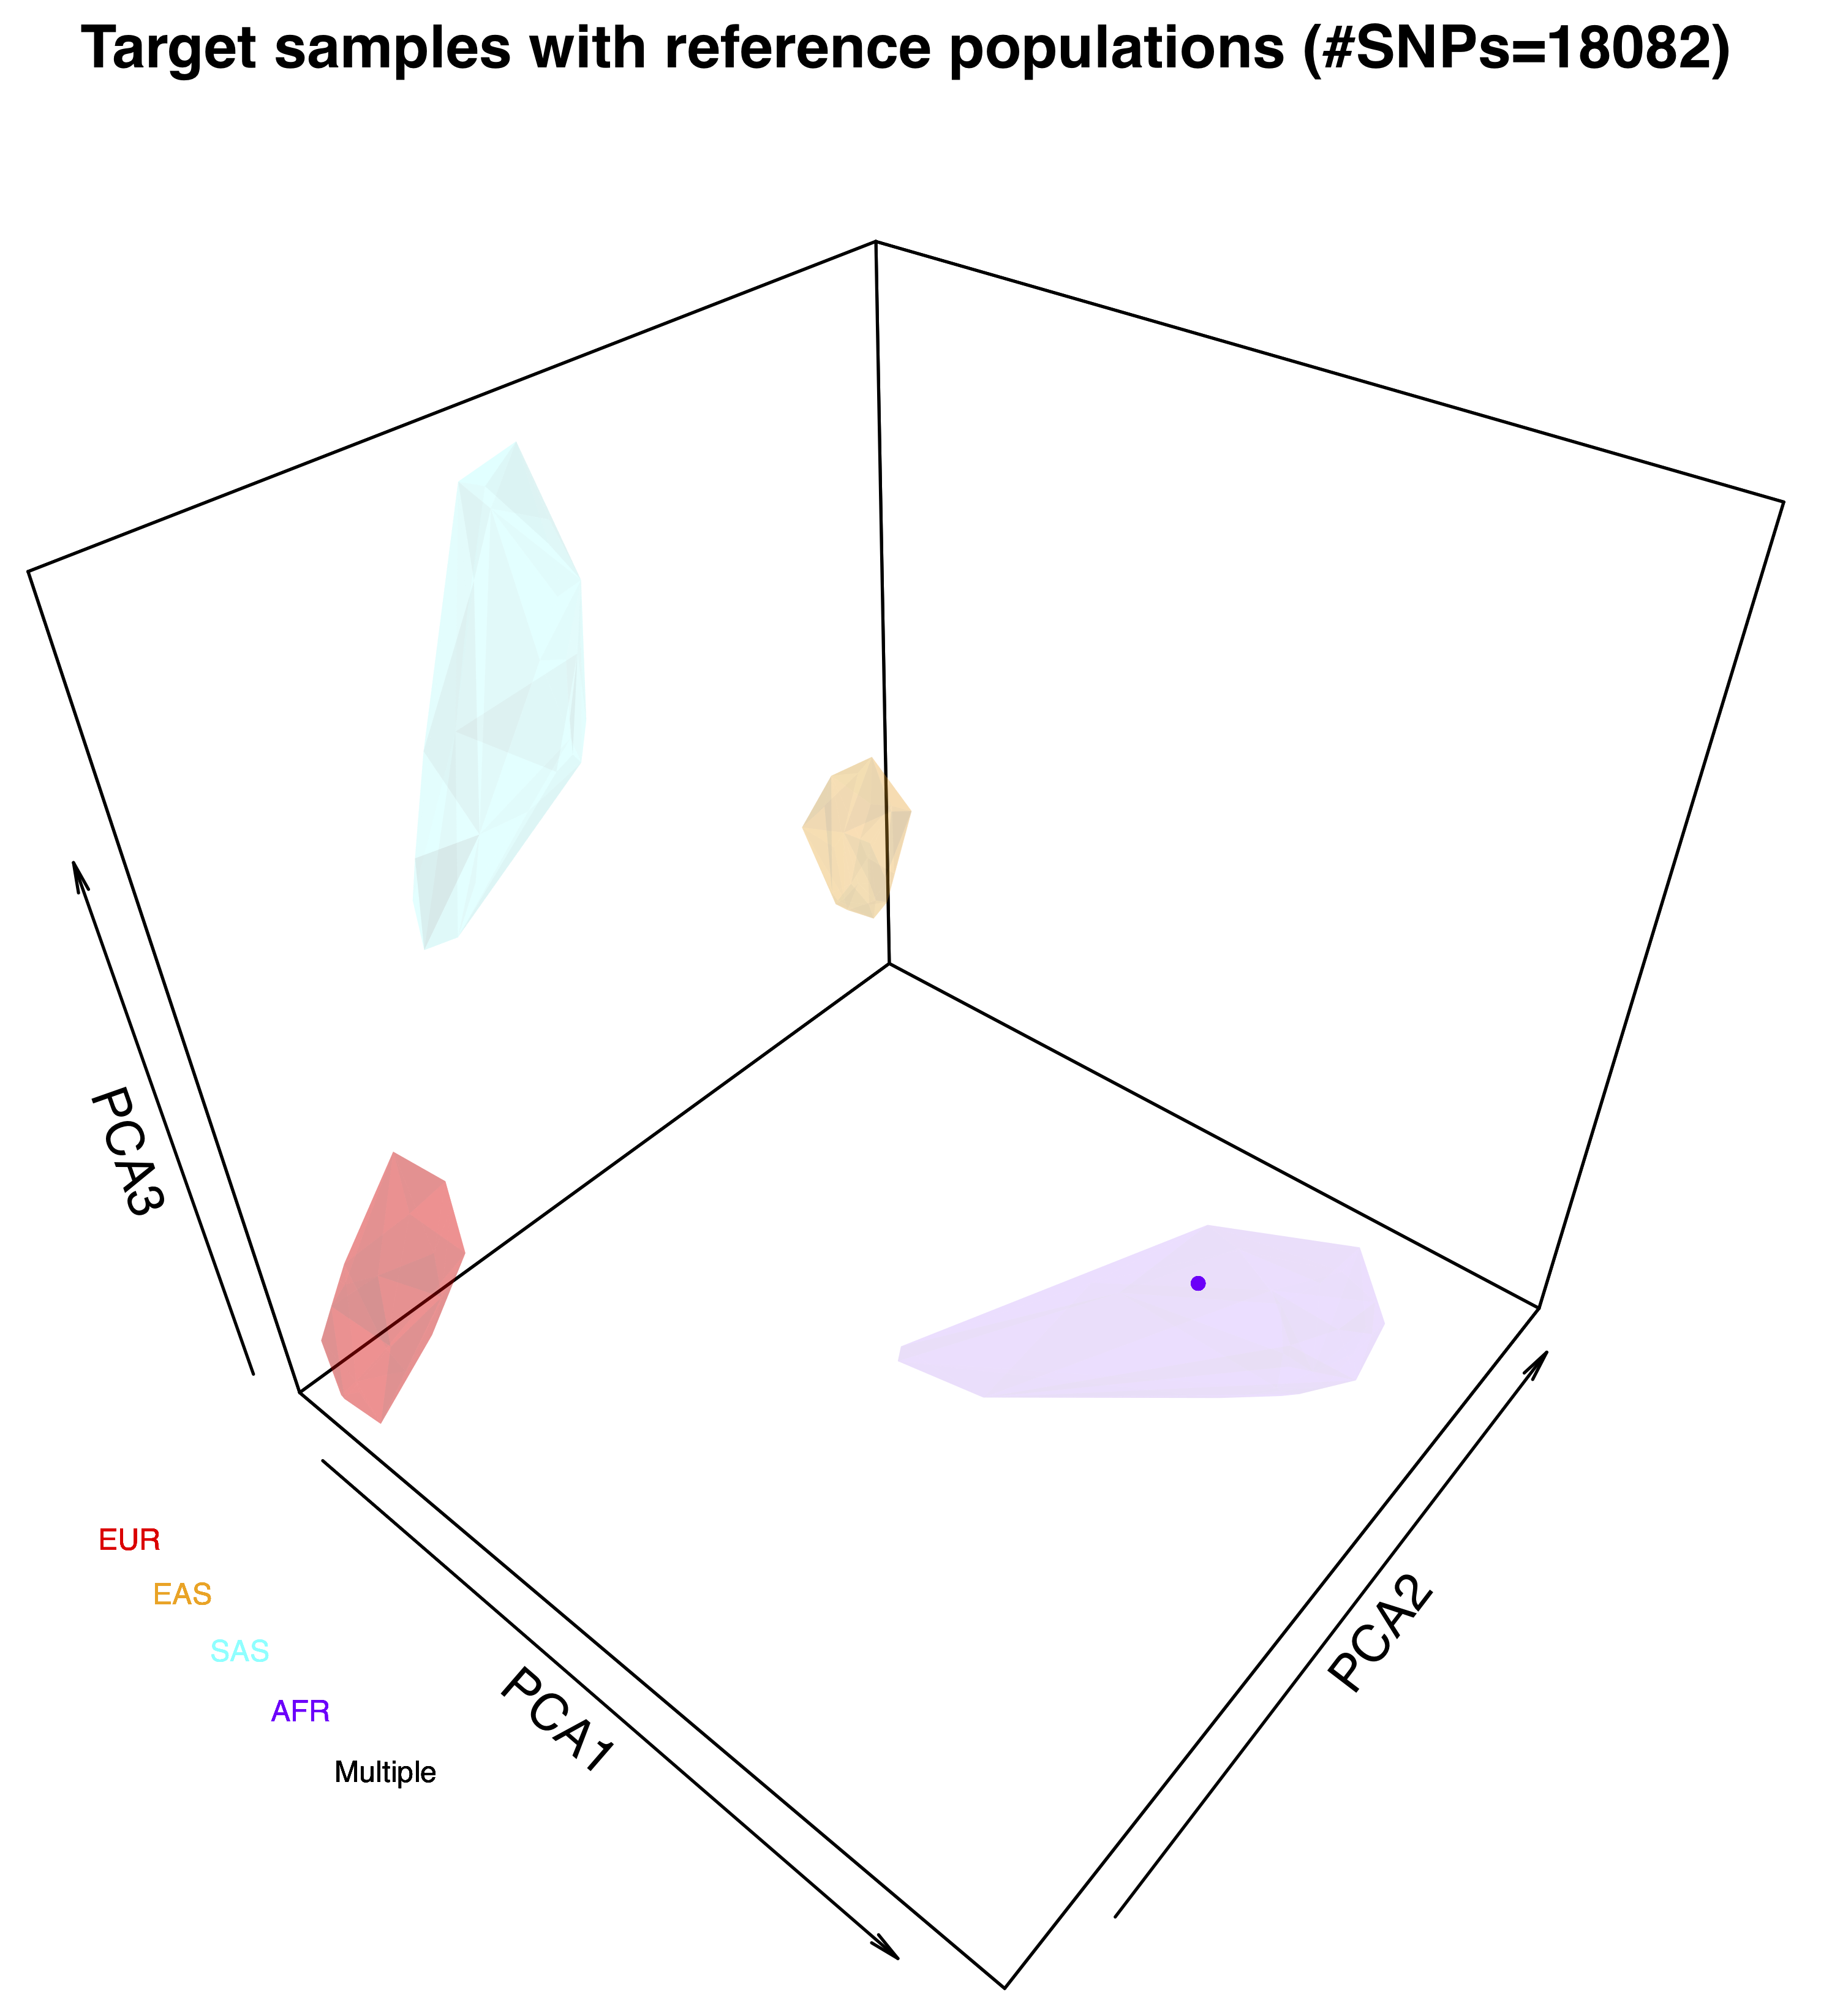
\includegraphics[width=0.5\textwidth]{images/EthSEQ_out.png}
   \caption{\footnotesize{EthSEQ output: the sample (purple dot) falls into the AFR area}}
   \label{ethSEQ}
\end{figure}

\paragraph{Somatic variant calling}

The results of the somatic copy-number calling are depicted in Figure \ref{fig:CBS}. Most of the segments present a log2 ratio value lower than zero, indicating that some deletions occurred. Since log2 ratio is measured as the base-2 logarithm of the tumor-related signal over the control signal, the expected value for heterozygous deletions is -1. However, due to confounding factors such as tumor purity and ploidy, the measured log2 ratios are likely to be shifted and it is safer to consider as heterozygous deletions the segments with values between -1.5 and -0.5. In particular, 101 out of 175 individuated segments present mean log2 ratio compatible with this kind of aberration. 

\begin{figure}[H]
\centering
    \centering
    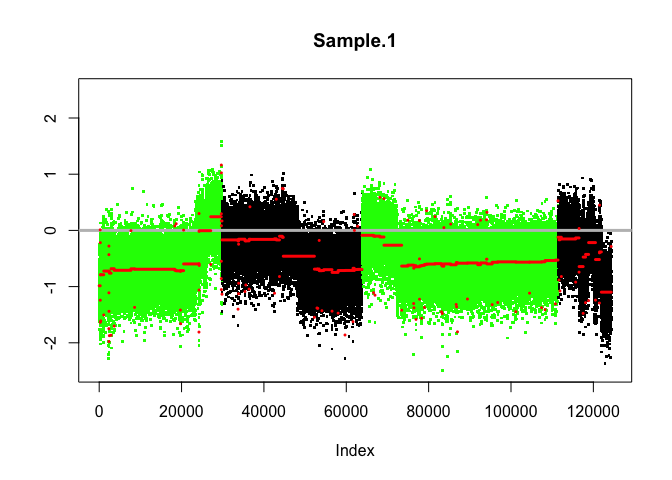
\includegraphics[width=0.8\linewidth]{images/SCNA_calling.png}
    \caption{\label{fig:CBS}\footnotesize{Circular binary segmentation results: red lines and dots indicate the mean log2 ratio of each segment, the colors divide the four analysed chromosomes.}}
\end{figure}

As for germline small variants, somatic point mutations were also called using two different tools. VarScan2 (setup 1) found 167 somatic point mutations, while Mutect2 (setup 2) found 641 point mutations; among them, 30 were found in common. An example of somatic point mutations found by Mutect2 in \emph{TP53} is reported in Figure \ref{pm_p53}. These low numbers are normal in this context since the BAM files from which variants were called represents only a small portion of the entire data belonging the original sample from TCGA. Also, significant differences in the number and types of variants identified are expected when comparing callset produced by different caller: piping them together is indeed a strategy to reduce the number of false negatives. Since Mutect2 claims to be more sensitive than other methods (especially for low allelic fraction and low read support events) while maintaining high specificity, we used this callset for the subsequent steps.


\paragraph{Variants in DNA repair genes}

If a DNA repair gene is characterized by the presence of small heterozygous variants associated with an increased risk of pathology, or even pathogenic ones, the accumulation of somatic aberrations in the copy number status (deletions, in particular) in those segments poses a significant threat with respect to the susceptibility to diseases. This seems to be what happened in this sample.
In fact, the only pathogenic variant identified in the callset of germline heterozygous SNPs is the one in \emph{BRCA1}, as already mentioned in the previous paragraph. Moreover, the intersection between segments with heterozygous deletions and DNA repair genes identified \emph{BRCA1} as one of the genes affected by the copy-number aberrations (Figure \ref{SCNA_DNARepair}). As can be seen in Figure \ref{igv_BRCA1}, the support for the alternative base (that encodes for the pathogenic SNP) is higher in the tumor sample harboring the somatic heterozygous deletion in \emph{BRCA1}: the combination of these aberrations is very likely related to the disease.

\begin{figure}[H]
   \centering
   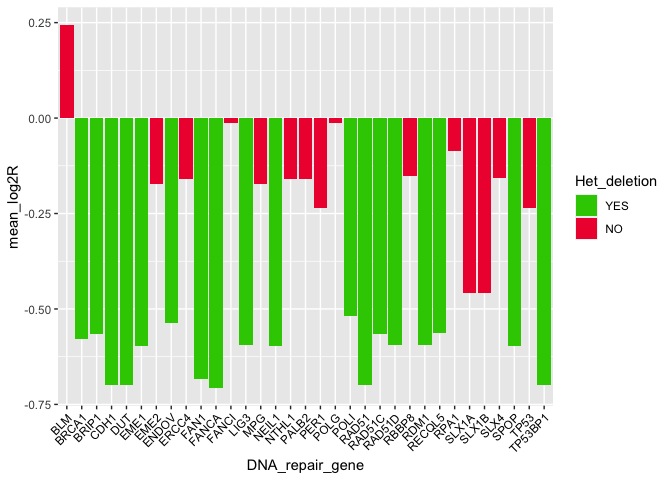
\includegraphics[width=0.5\textwidth]{images/SCNA_DNARepairGenes.png}
   \caption{\footnotesize{Mean log2Ratio of segments containing DNA repair genes}}
   \label{SCNA_DNARepair}
\end{figure}

By intersecting the entire callset of germline SNPs (found with the setup 2, instead of considering only the clinically significant one) with the newly generated .bed file containing the DNA repair genes with heterozygous deletions (see methods), a higher number of variants were individuated (figure \ref{germline_dna_repair}). However, it is likely that these variants do not affect greatly the patient's conditions, since none of them were annotated as pathogenic by Clinvar. They can still be associated to disease susceptibility, although this cannot be concluded without further annotation data.

The same workflow was applied to the somatic variant callset (from Mutect, setup 2), this time without considering the clinical relevance and dividing the callset into indels and point mutations; the number of variants with respect to each DNA repair gene (harboring an heterozygous deletion) are reported in Figure \ref{somatic_dna_repair}. 

\begin{figure}[H]
\centering
\begin{subfigure}{.47\textwidth}
    \centering
    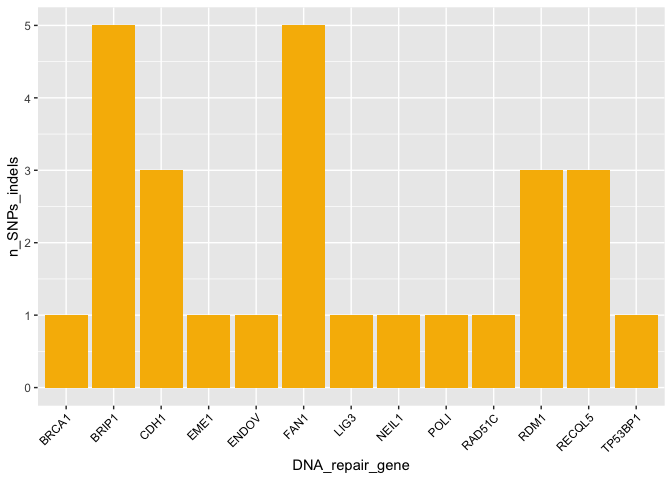
\includegraphics[width=\linewidth]{images/overlap_germline.png}
    \caption{\label{germline_dna_repair}\footnotesize{Number of germline heterozygous variants found across DNA repair genes that underwent a somatic heterozygous deletion. Since only the SNP in BRCA1 was found to be pathogenic, all the callset was used to find the number of germline small variants within each DNA repair gene.}}
\end{subfigure}
\hfill                      
\begin{subfigure}{.47\textwidth}
    \centering
    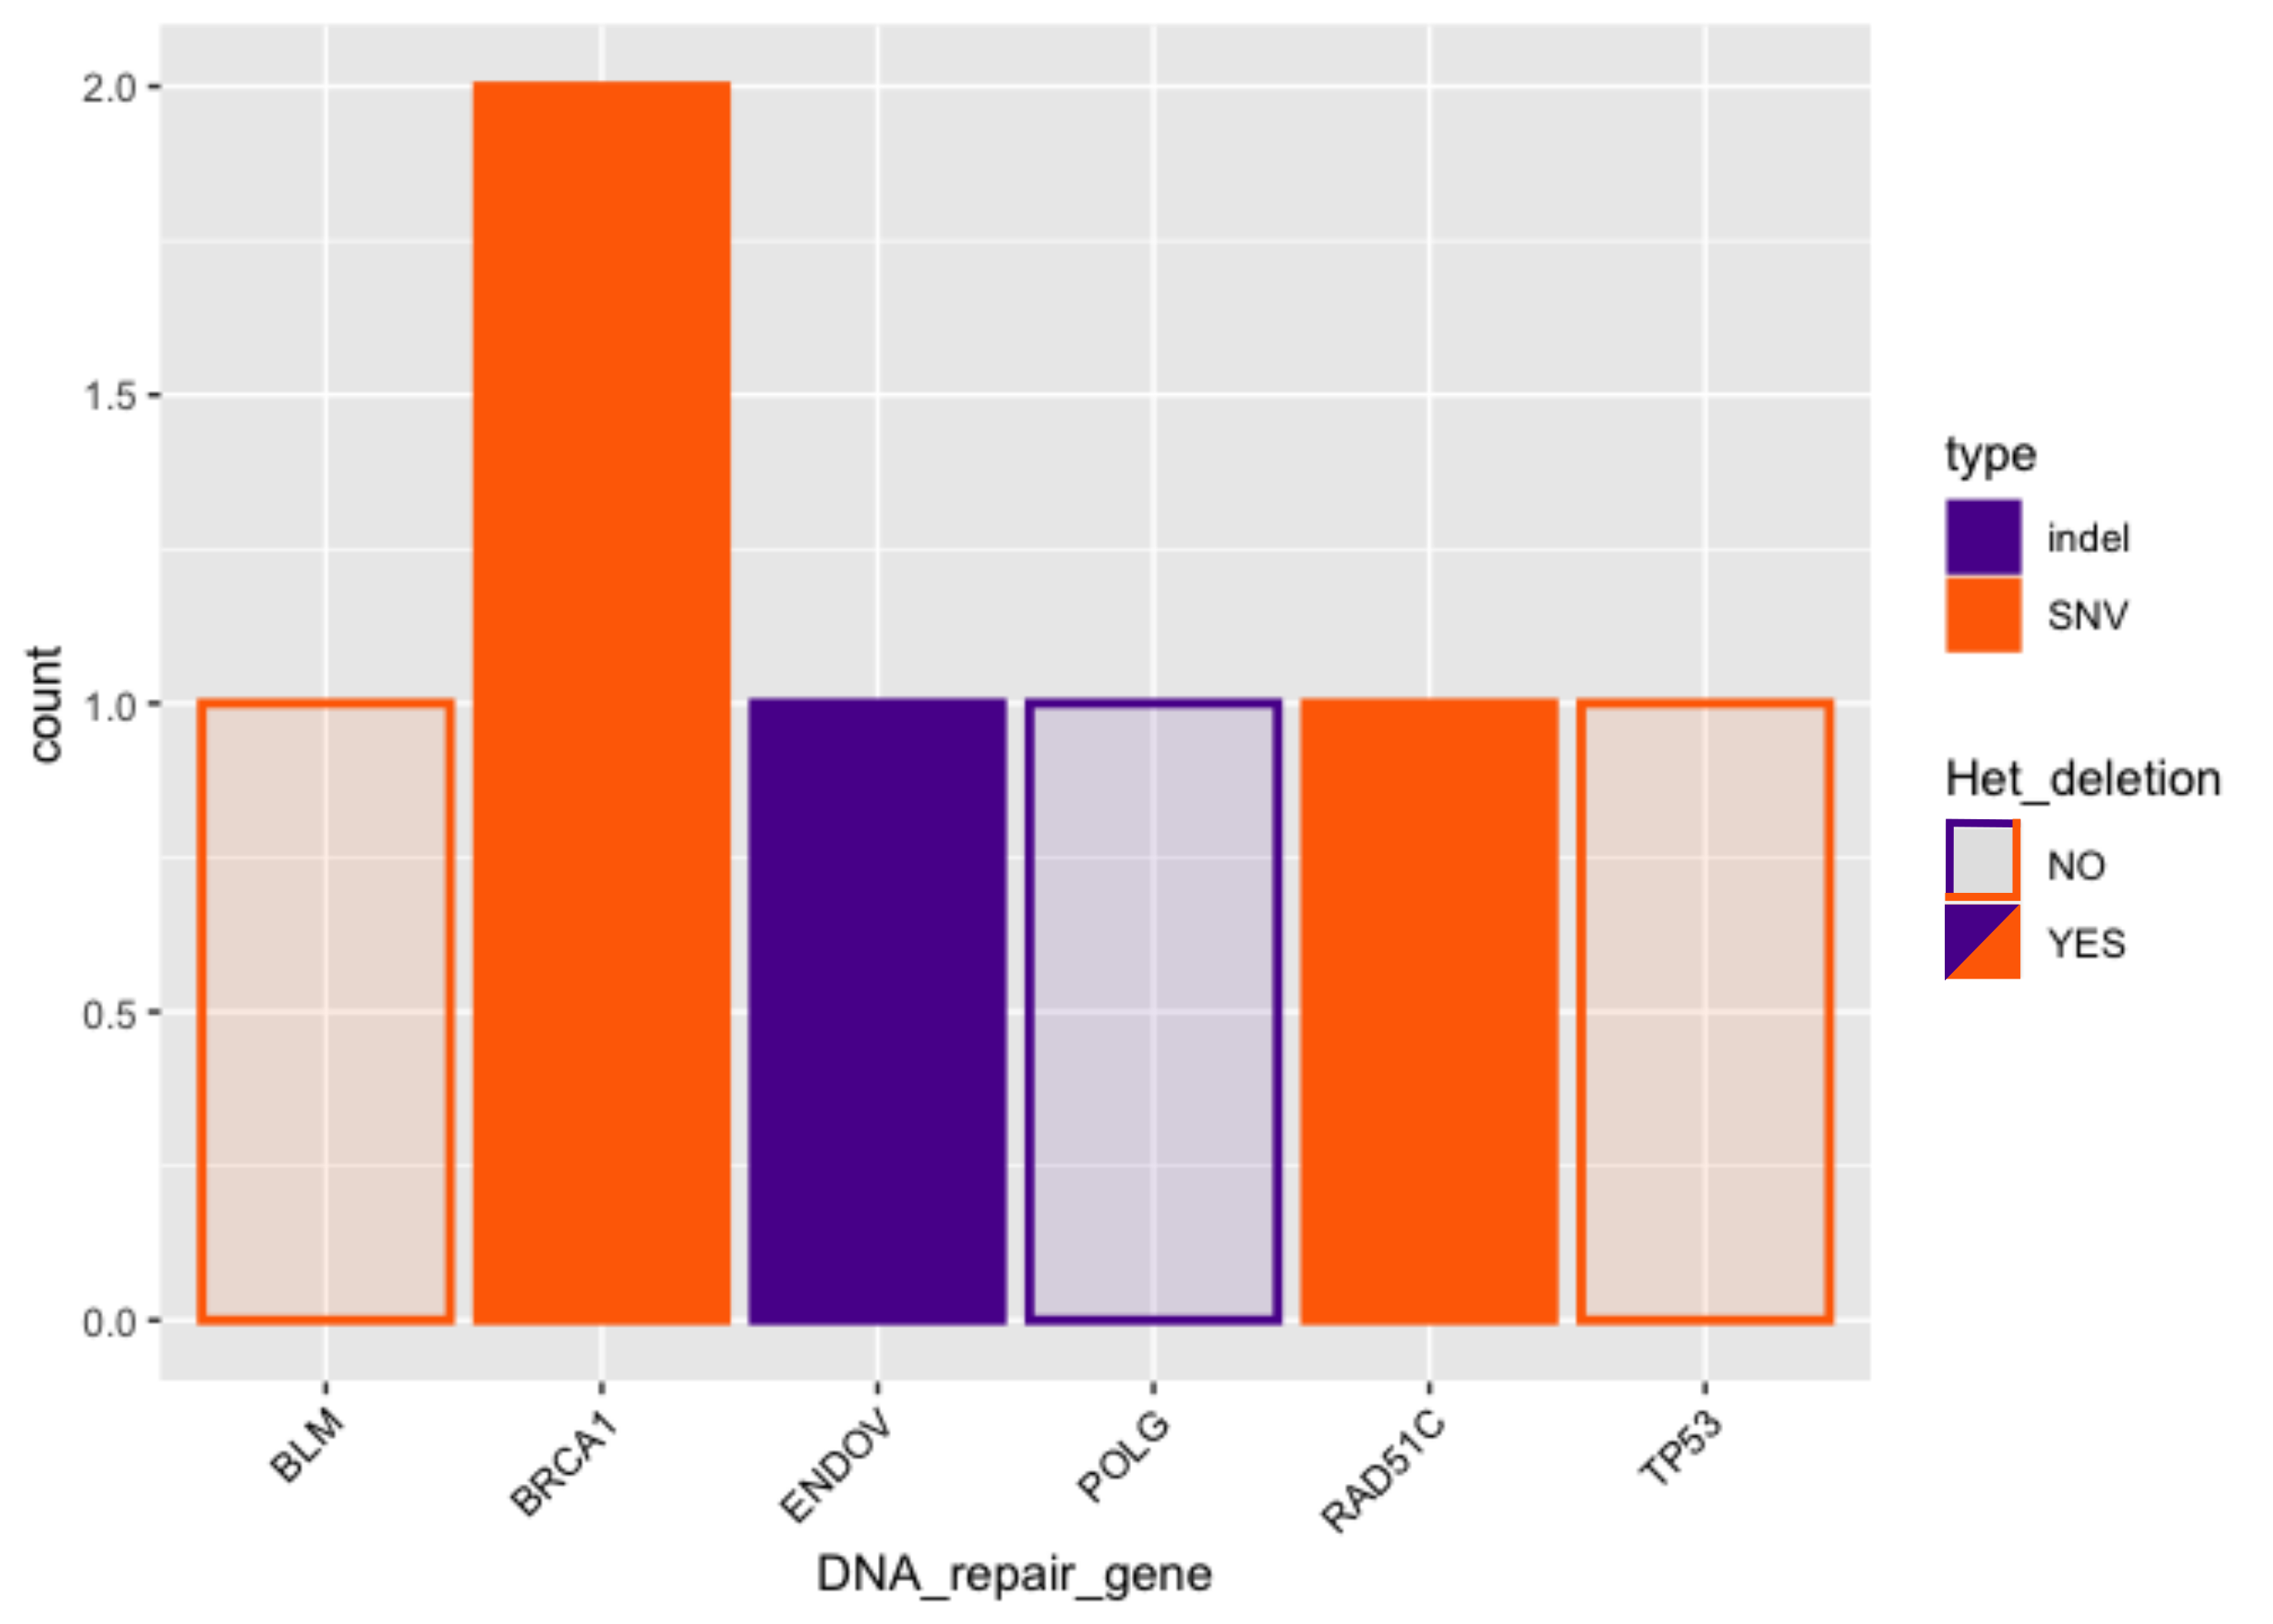
\includegraphics[width=\linewidth]{images/overlap_somatic.png}
    \caption{\label{somatic_dna_repair}\footnotesize{Number of somatic point mutations and indels found in DNA repair genes that harbor a somatic heterozygous deletion}}
\end{subfigure}
\caption{\footnotesize{DNA repair genes overlaps with variants.}}
\end{figure}


\paragraph{Tumor purity and ploidy}

Tumor ploidy and admixture computed with \texttt{CLONETv2} resulted of respectively 2.24 and 0.36. Consequently, the estimated tumor purity is 0.64. The log2 ratio values for each considered variant, obtained in the previous section, were plotted against the newly-calculated beta values to better discriminate between different copy-number alterations.

As confirmation of the previous results, a large number of the considered segments fall into a segment with heterozygous deletion, indicated in the figure \ref{clonet} by the label \textit{(1,0)} representing the copy-number of the major and minor alleles. Allele-specific copy-numbers are represented clearly in the supplementary figure \ref{cn}.

In contrast, the analysis carried out with \texttt{TPES} produced different results, with an estimation of tumor purity equal to 0.94. However, as stated by the \texttt{TPES} results summary (\ref{tpes}), only 11 SNVs were considered for this step, a number far too small to have a reliable purity estimation. Moreover, it was observed that this result is quite variable depending on the threshold set on the reference mapping bias (by default set at RMB=0.47).


\begin{figure}[H]
\centering
\begin{subfigure}{.47\textwidth}
    \centering
    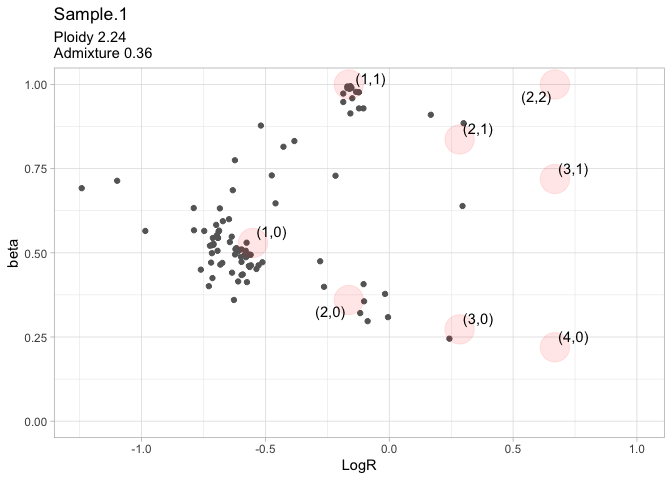
\includegraphics[width=\linewidth]{images/check_plot.png}
    \caption{\label{clonet}\footnotesize{CLONET results: beta values plotted over the normalized log2 ratio values for each segment}}
\end{subfigure}
%
\begin{subfigure}{.47\textwidth}
    \centering
    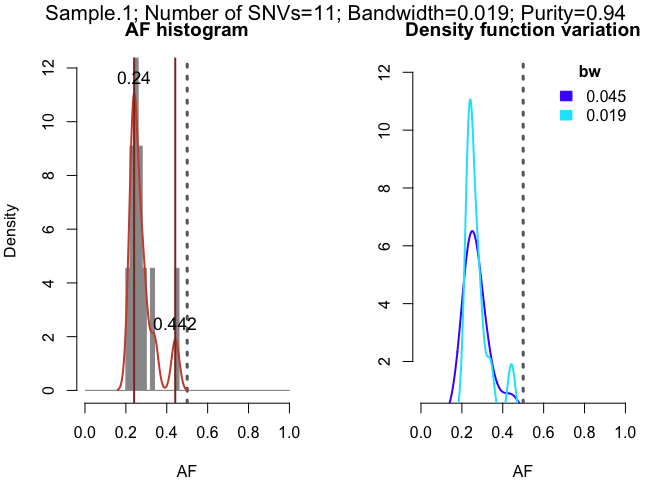
\includegraphics[width=\linewidth]{images/TPES.png}
    \caption{\label{tpes}\footnotesize{TPES results: the first picture shows allelic fraction distribution of putative clonal and subclonal SNVs within copy-number neutral segments}}
\end{subfigure}
\caption{\footnotesize{Tumor purity and ploidy estimation}}
\end{figure}


\paragraph{SPIA analysis}

SPIA analysis was performed considering the SNPs of the hapmap file which were in common between the tumor and control and gave as result a distance of 0.18809 between the samples, classified as \textit{uncertain}. This score was expected to be low, since both samples come from the same patient. The uncertainty is probably given by the mutations found in the tumor cells, that bring some difference between the two.


\section*{Conclusions}

Our study was aimed at identifying and characterizing germline and somatic variants, determining the ancestry of the patient, and study the tumor ploidy and purity of a provided breast cancer sample retrieved from TCGA. 
First, we were able to properly pre-process the given data, following the requirements of different callers; then, both legacy tools and best-practice ones were used to call germline SNPs, somatic CNVs and somatic point mutations. Second, by intersecting the obtained information, we were able to properly assess the status of a pathogenic variant (in \emph{BRCA1}) associated with the tumor that the patient suffers from, linking the presence of this germline heterozygous variant with a subsequent somatic heterozygous deletion. Finally, the tumor sample was characterized in its purity, and the ploidy of the tumor was computed.

% Small files and already preprocessed







\clearpage

\appendix
\renewcommand{\thefigure}{S\arabic{figure}}
\setcounter{figure}{0}


\section*{Supplementary Figures}

\begin{figure}[h]
   \centering
   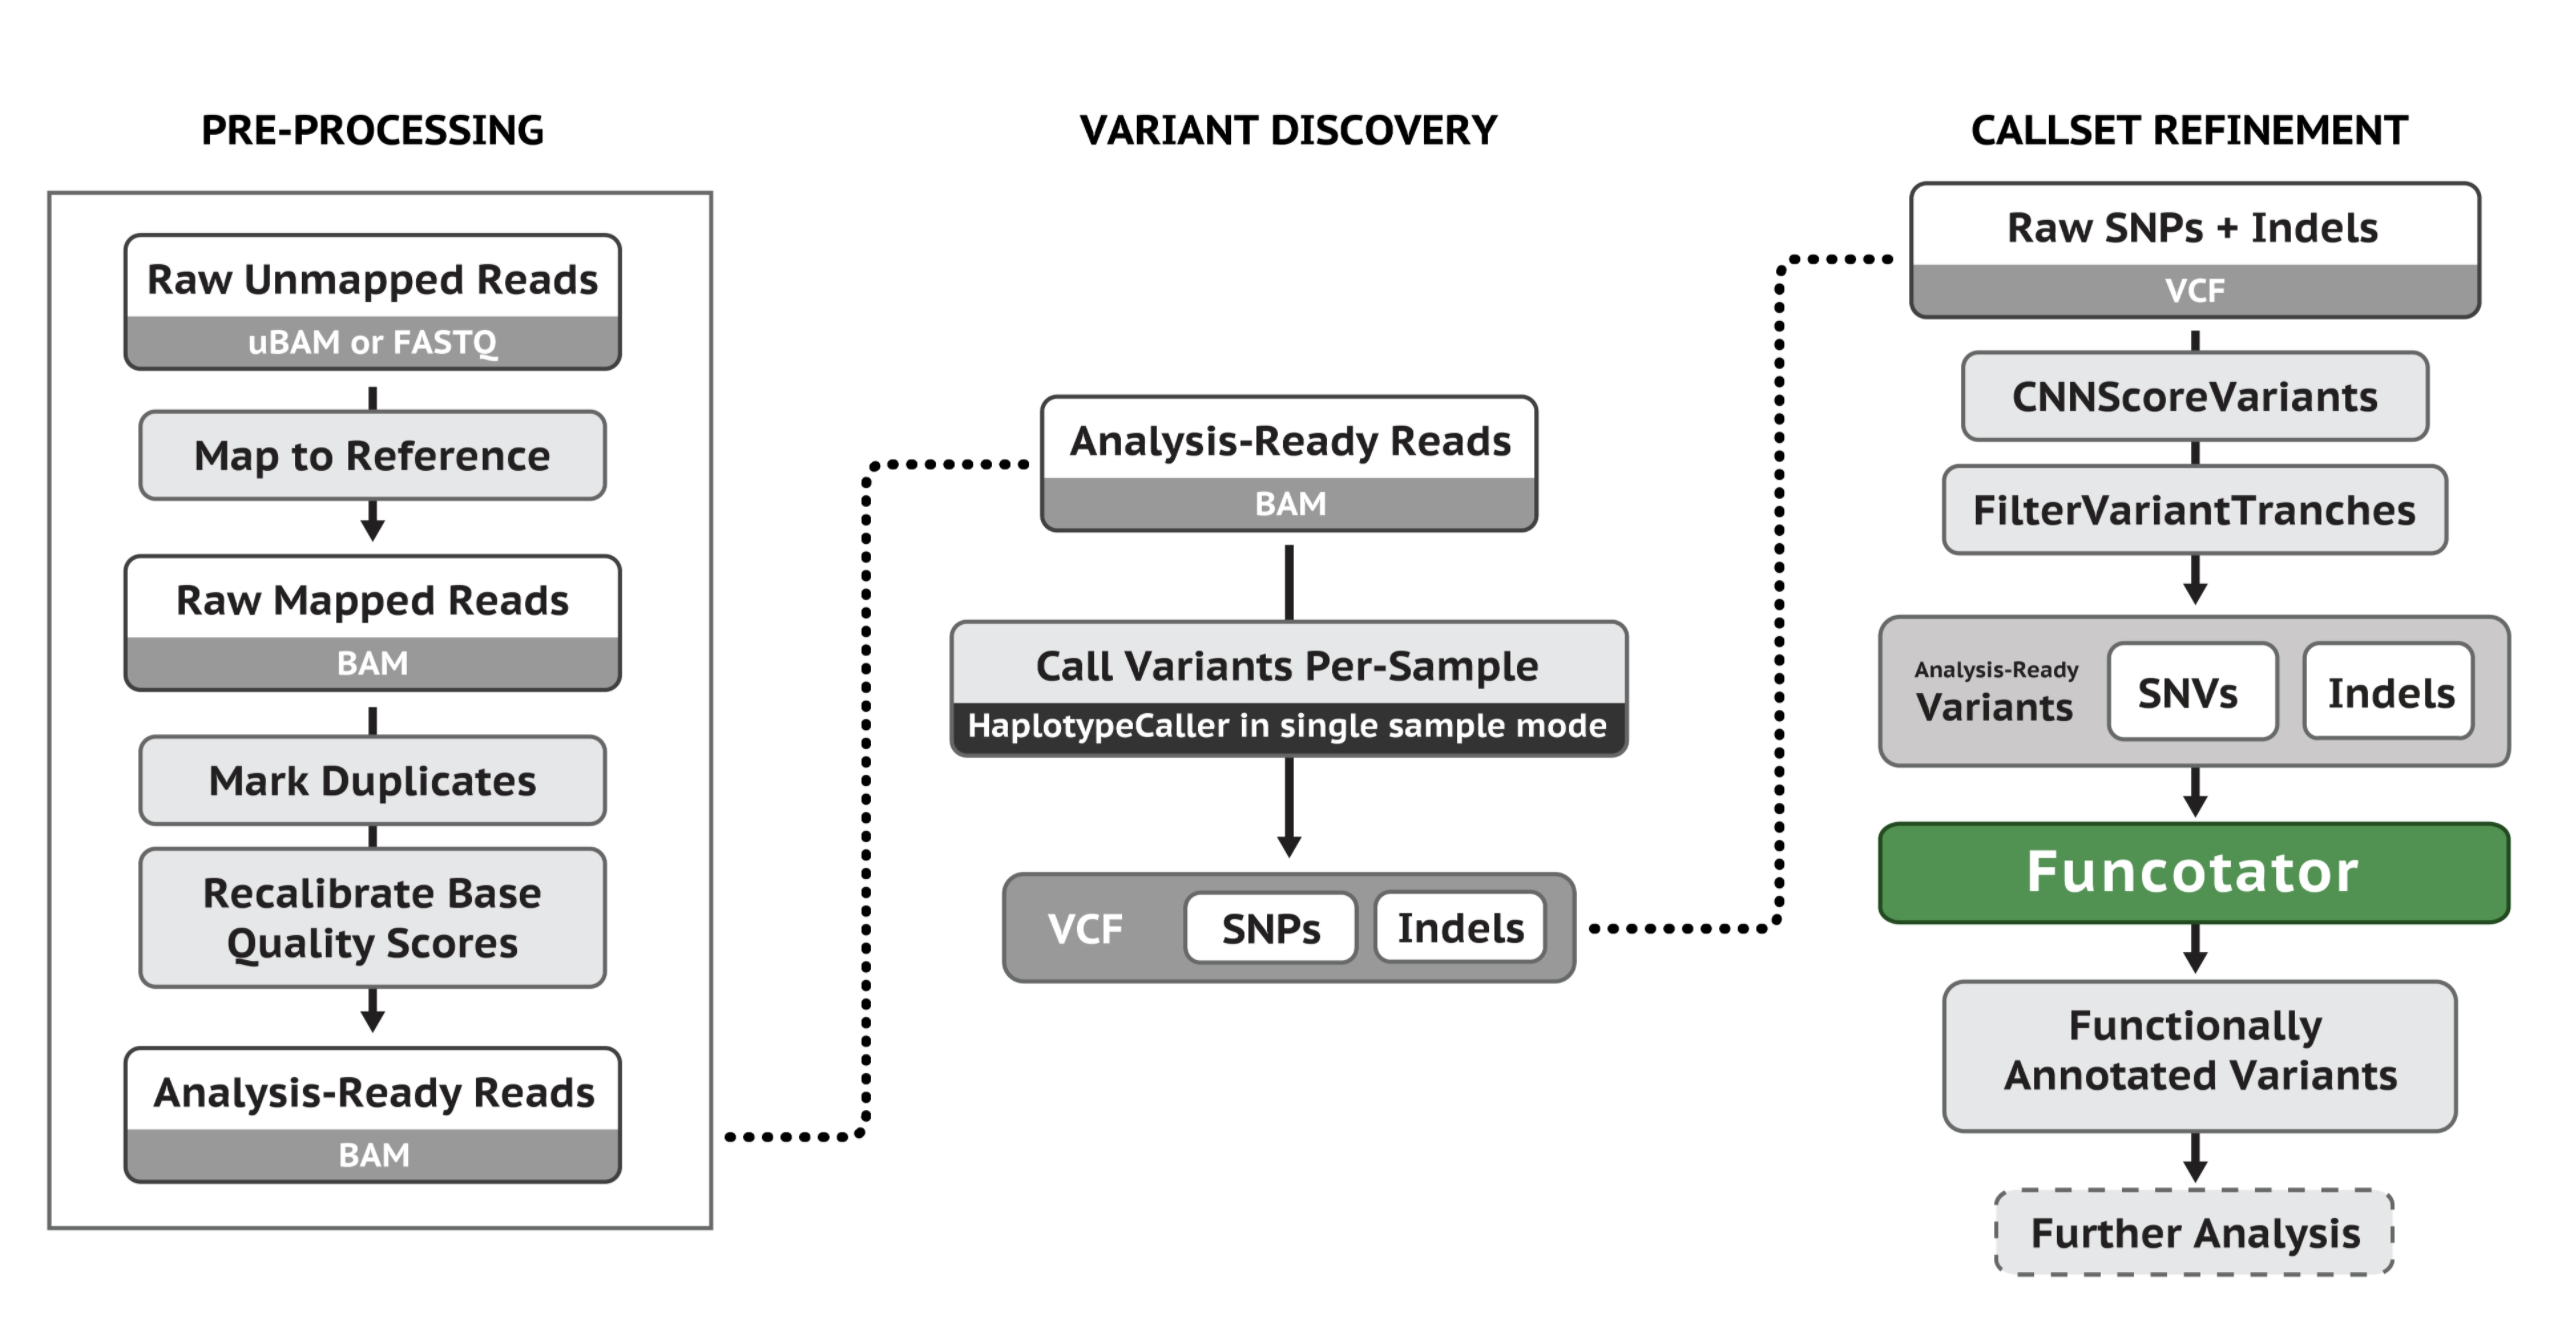
\includegraphics[width=0.8\textwidth]{images/variant_calling_pipeline.png}
   \caption{\footnotesize{Best-practice workflow for small germline variant discovery taken from GATK website \href{https://gatk.broadinstitute.org/hc/en-us/articles/360035535932}{(link)} }}
   \label{pipeline_germline_variant}
\end{figure}


\begin{figure}[h]
   \centering
   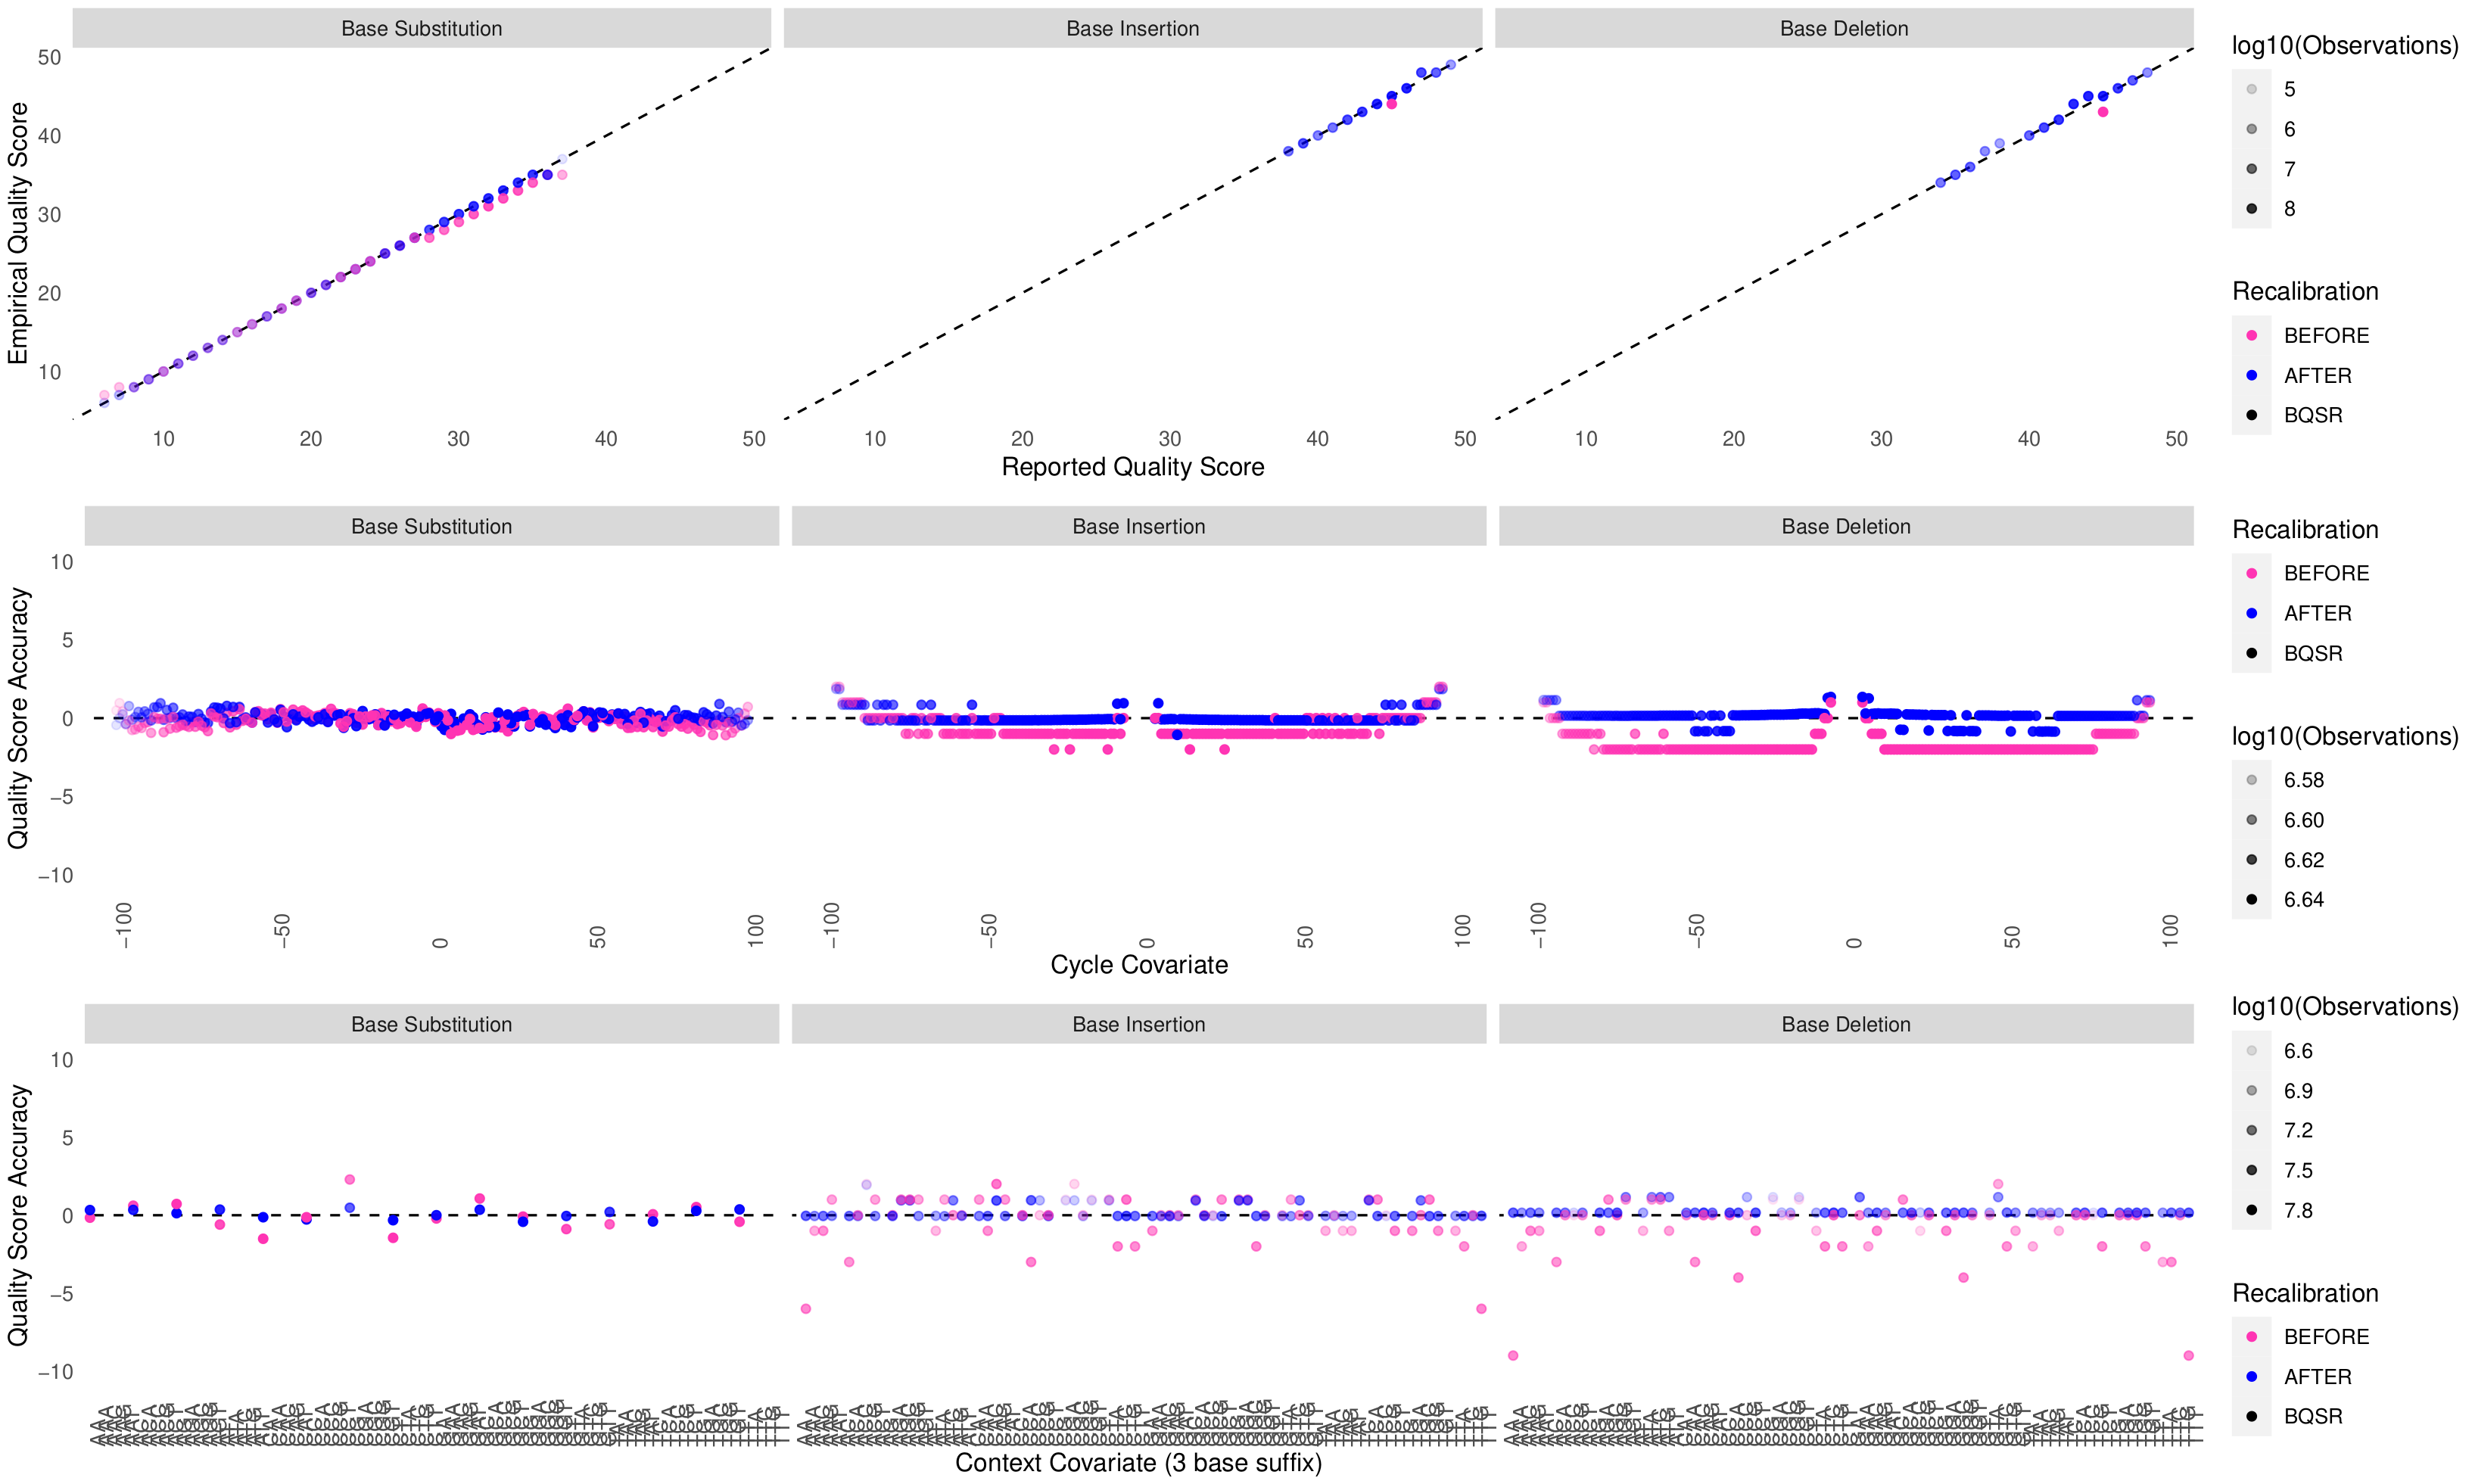
\includegraphics[width=\textwidth]{images/recal_control_1_setup1.png}
   \caption{\footnotesize{Recalibration control sample}}
   \label{recal_control_1}
\end{figure}

\begin{figure}[h]
   \centering
   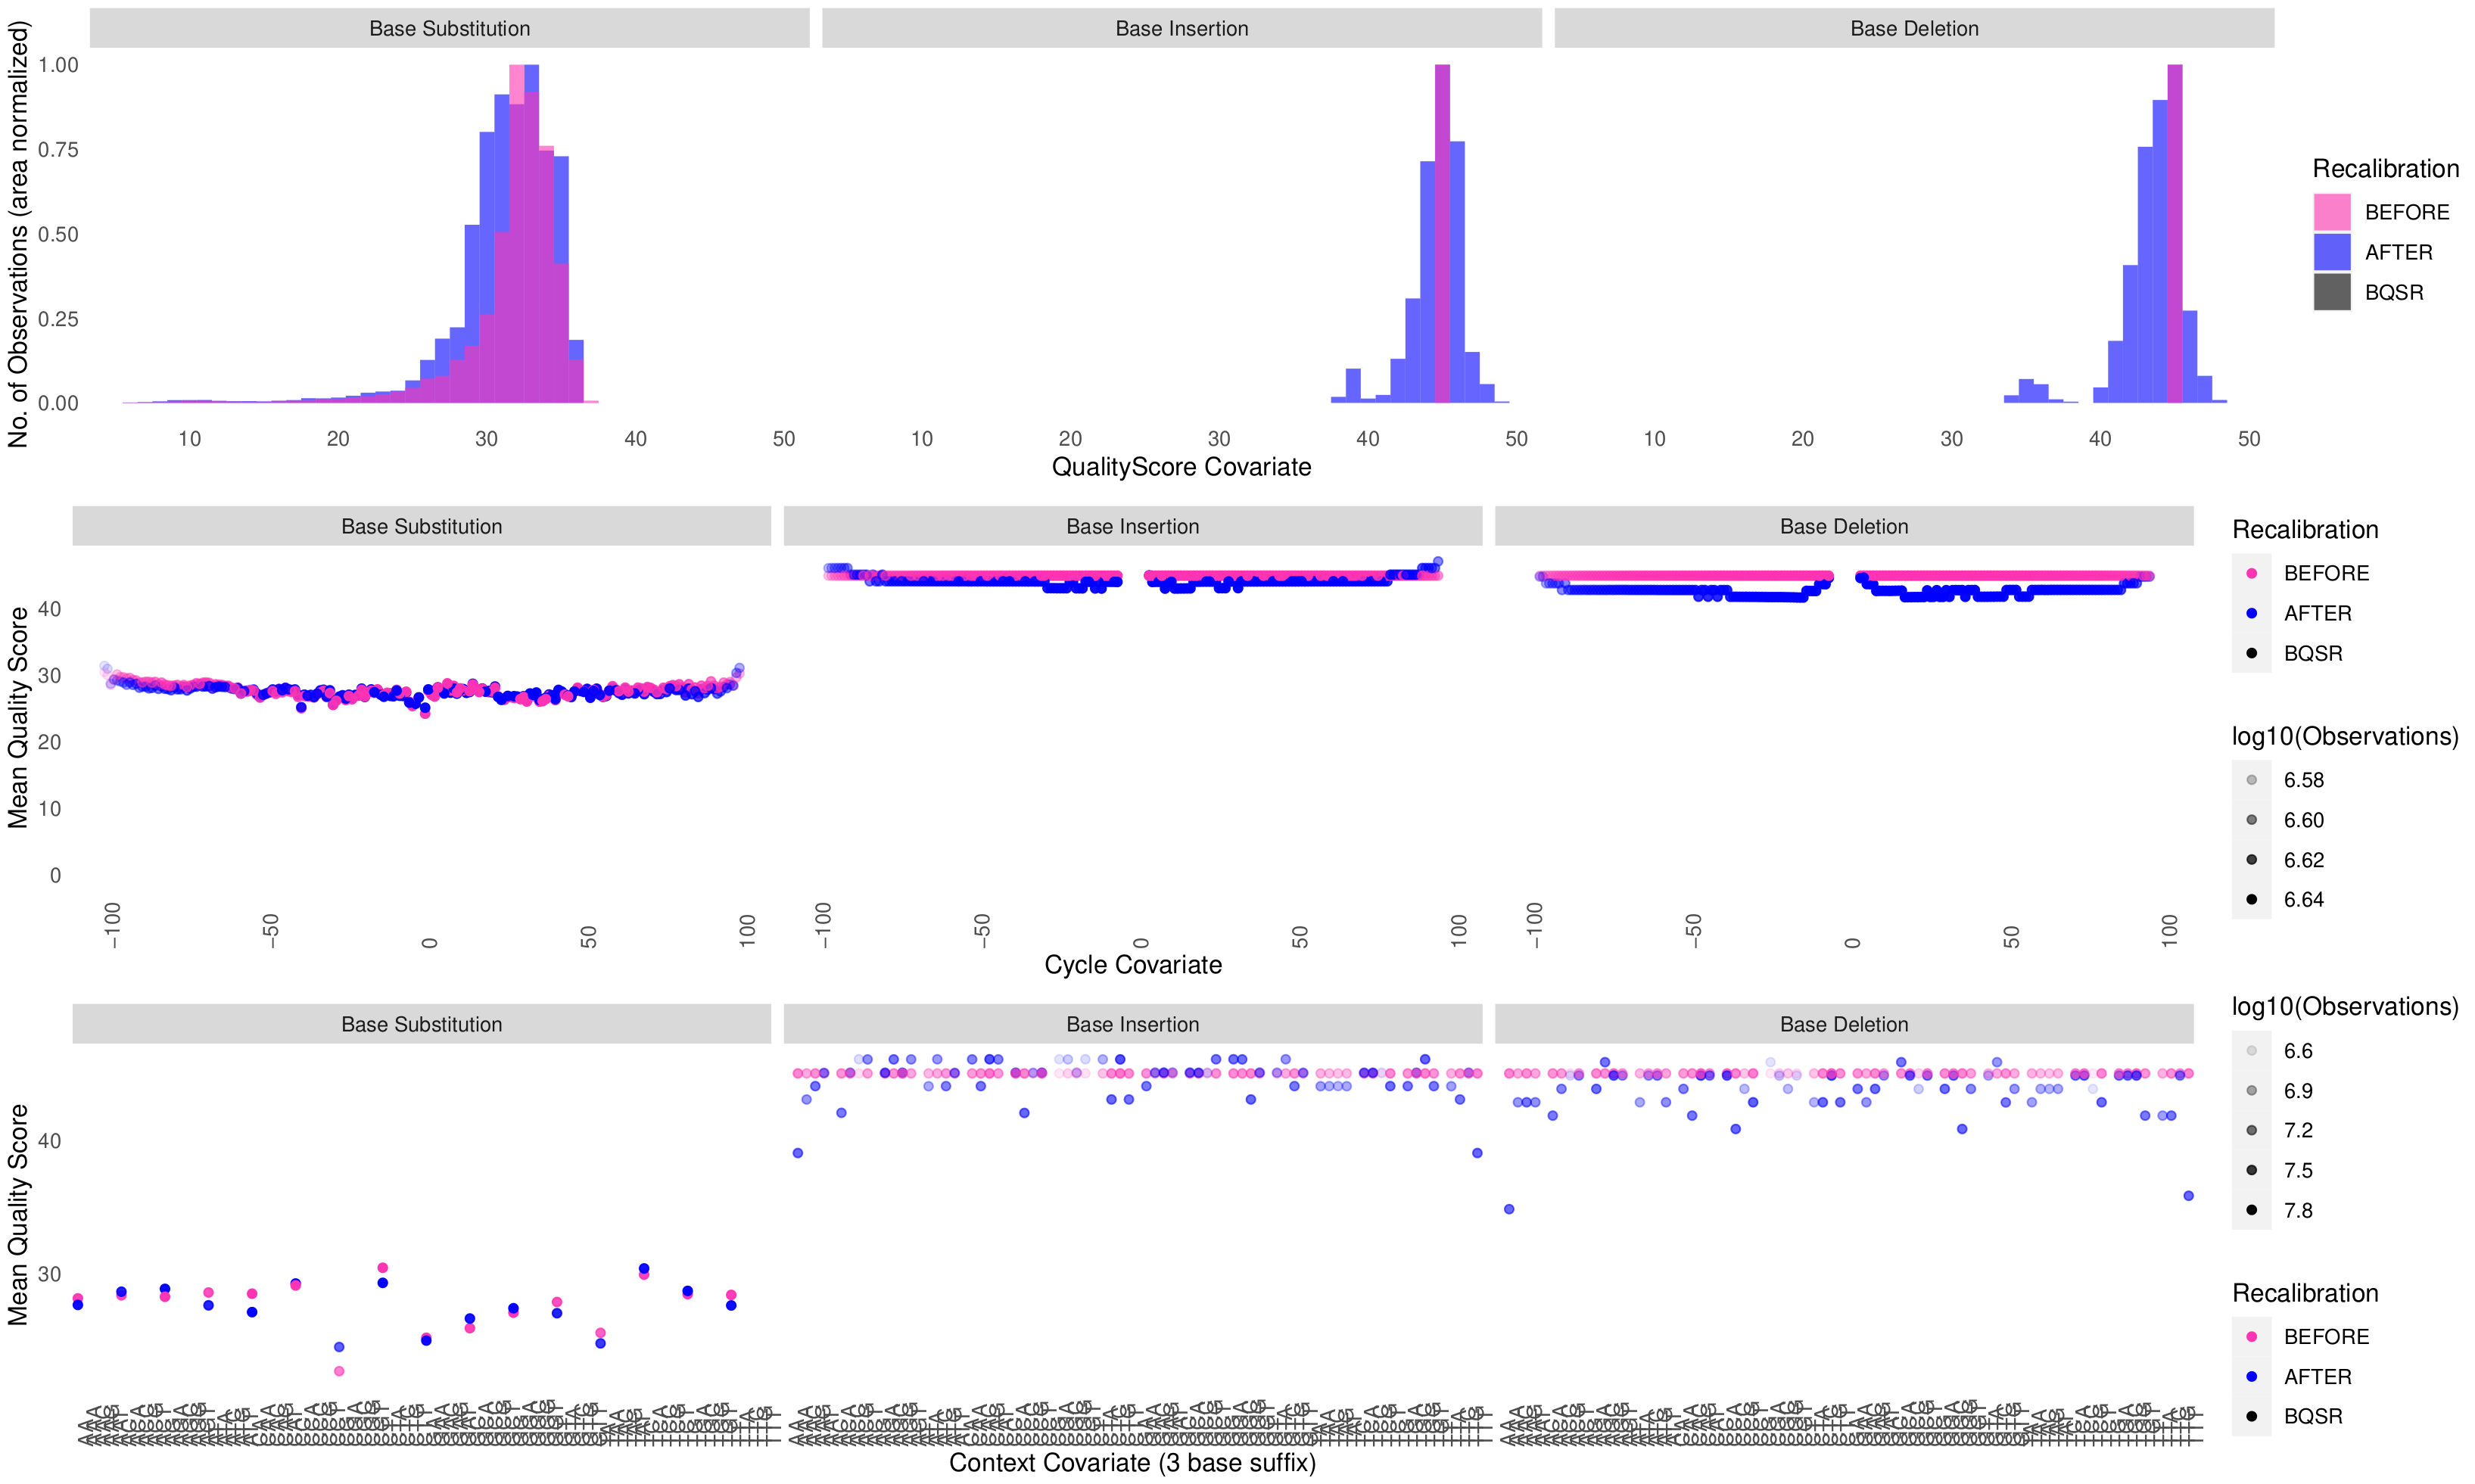
\includegraphics[width=\textwidth]{images/recal_control_2_setup1.png}
   \caption{\footnotesize{Recalibration control sample}}
   \label{recal_control_2}
\end{figure}

\begin{figure}[h]
   \centering
   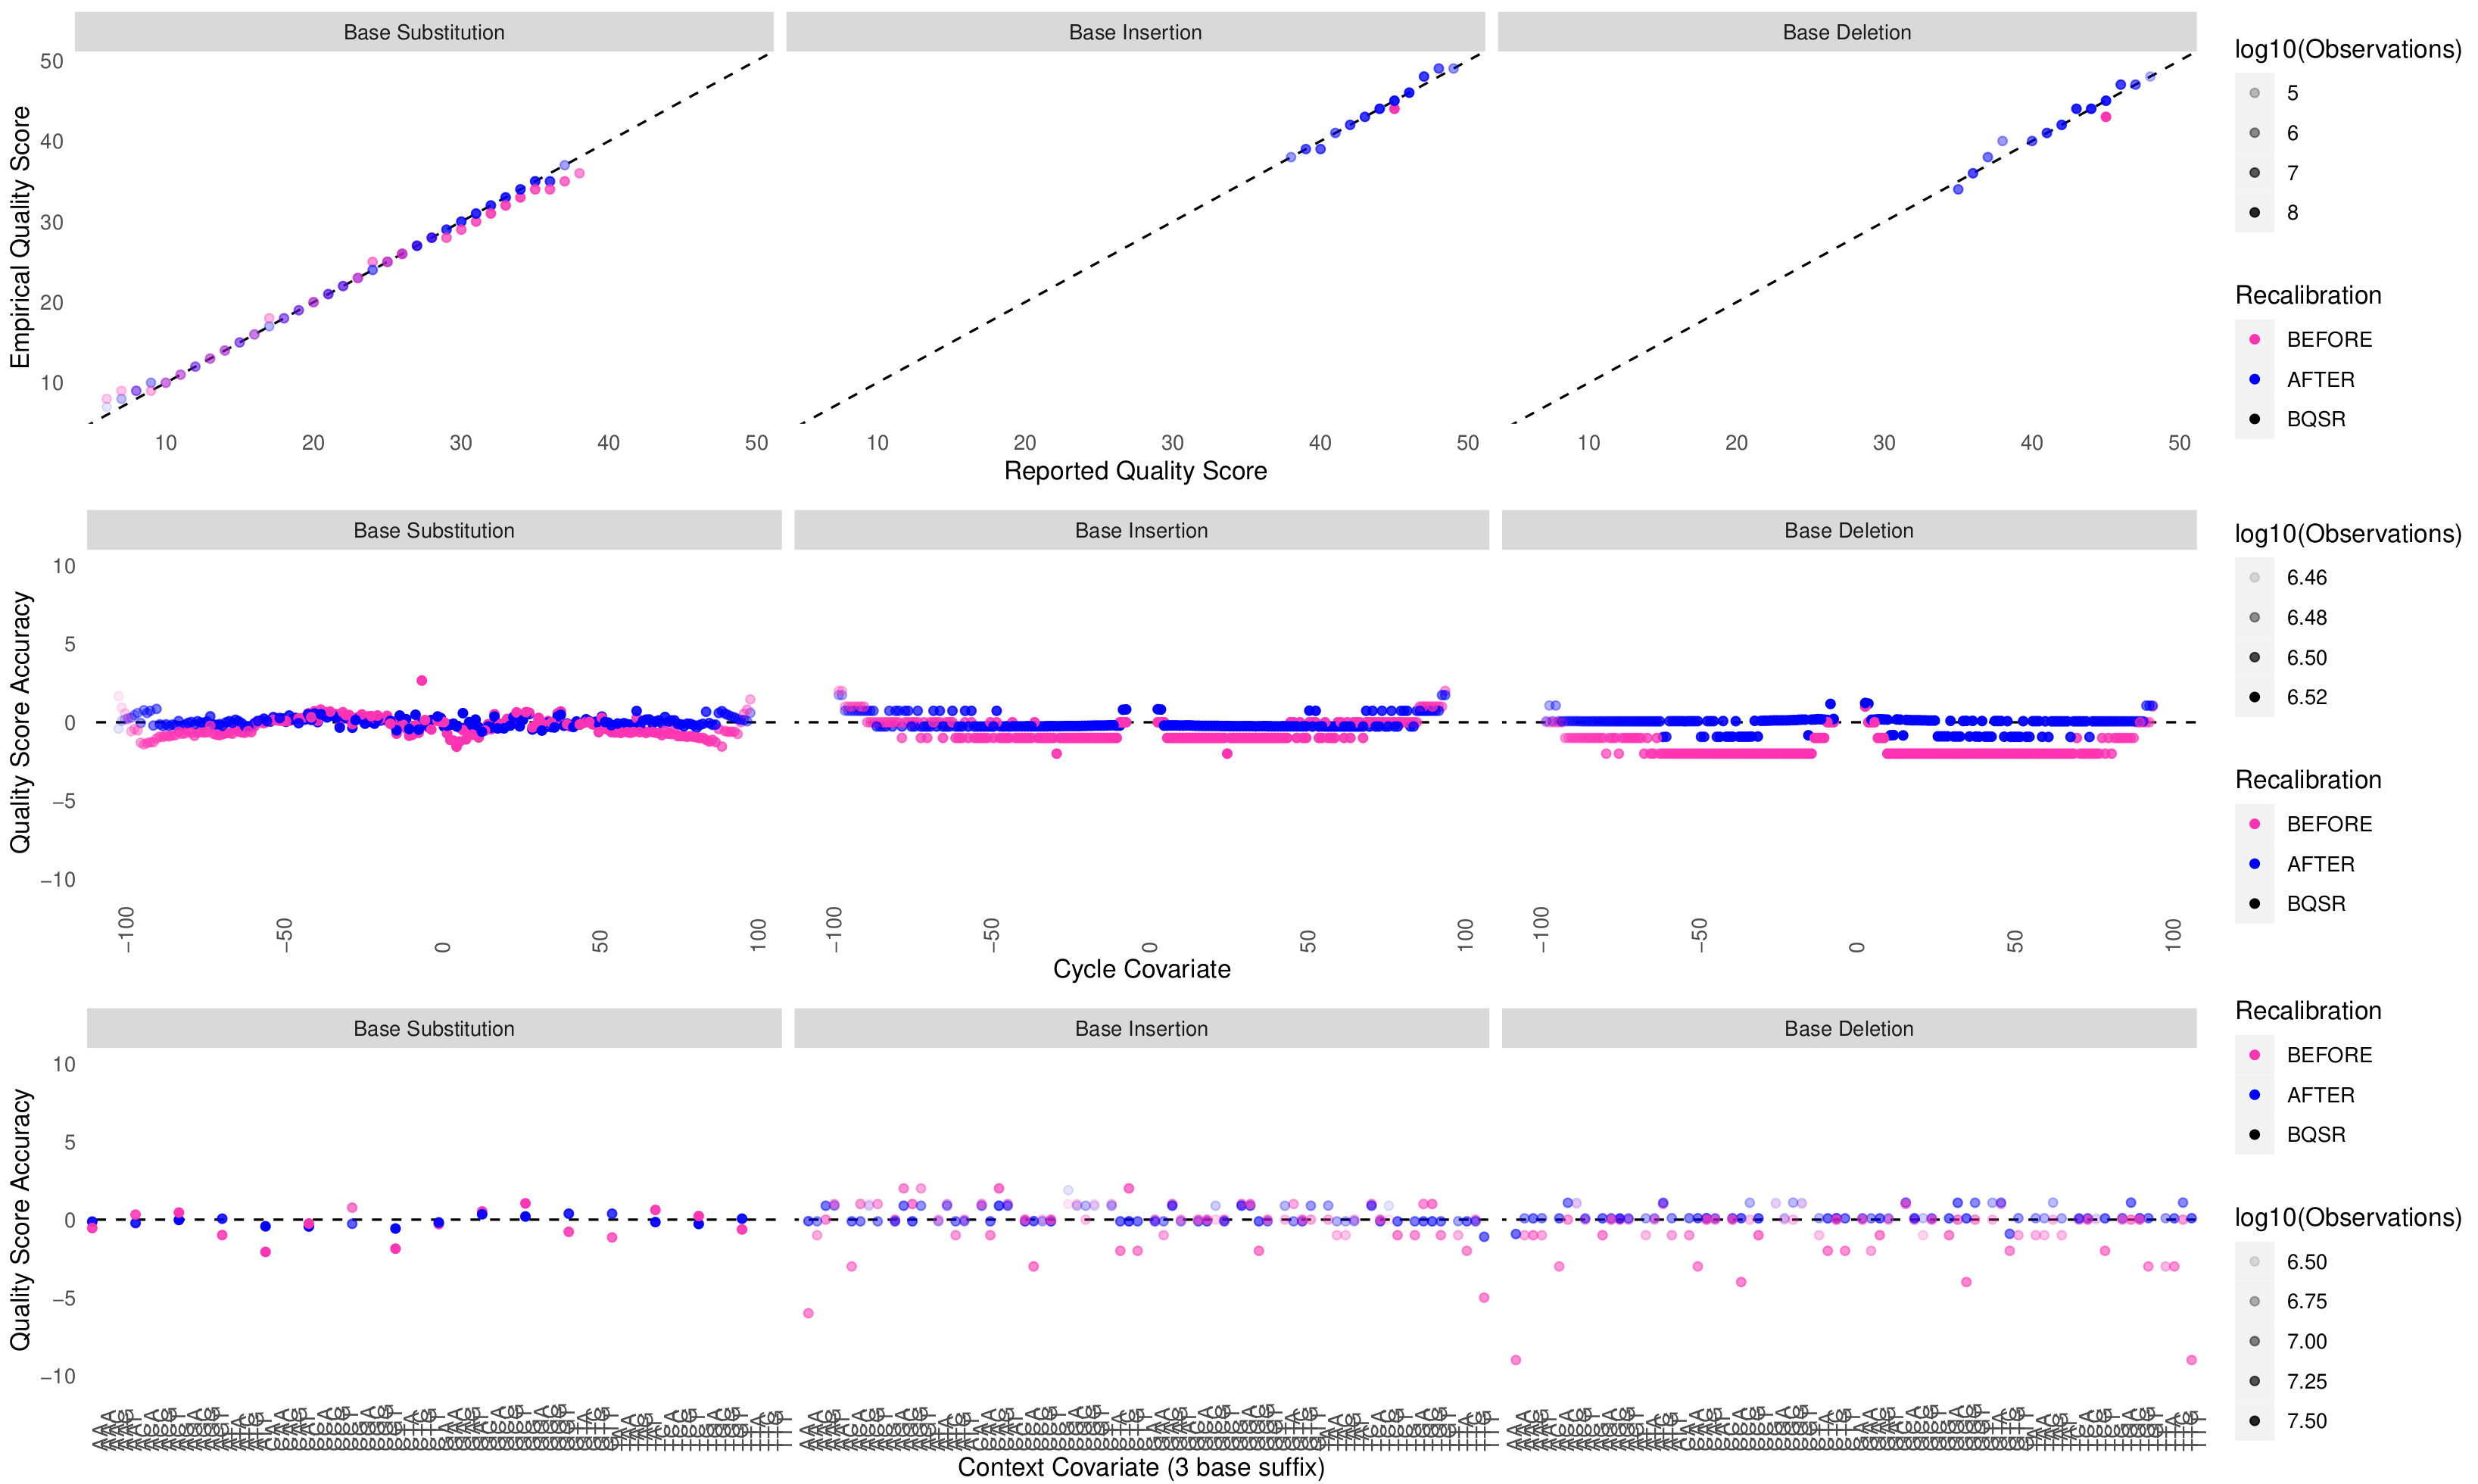
\includegraphics[width=\textwidth]{images/recal_tumor_1_setup1.png}
   \caption{\footnotesize{Recalibration tumor sample}}
   \label{recal_tumor_1}
\end{figure}

\begin{figure}[h]
   \centering
   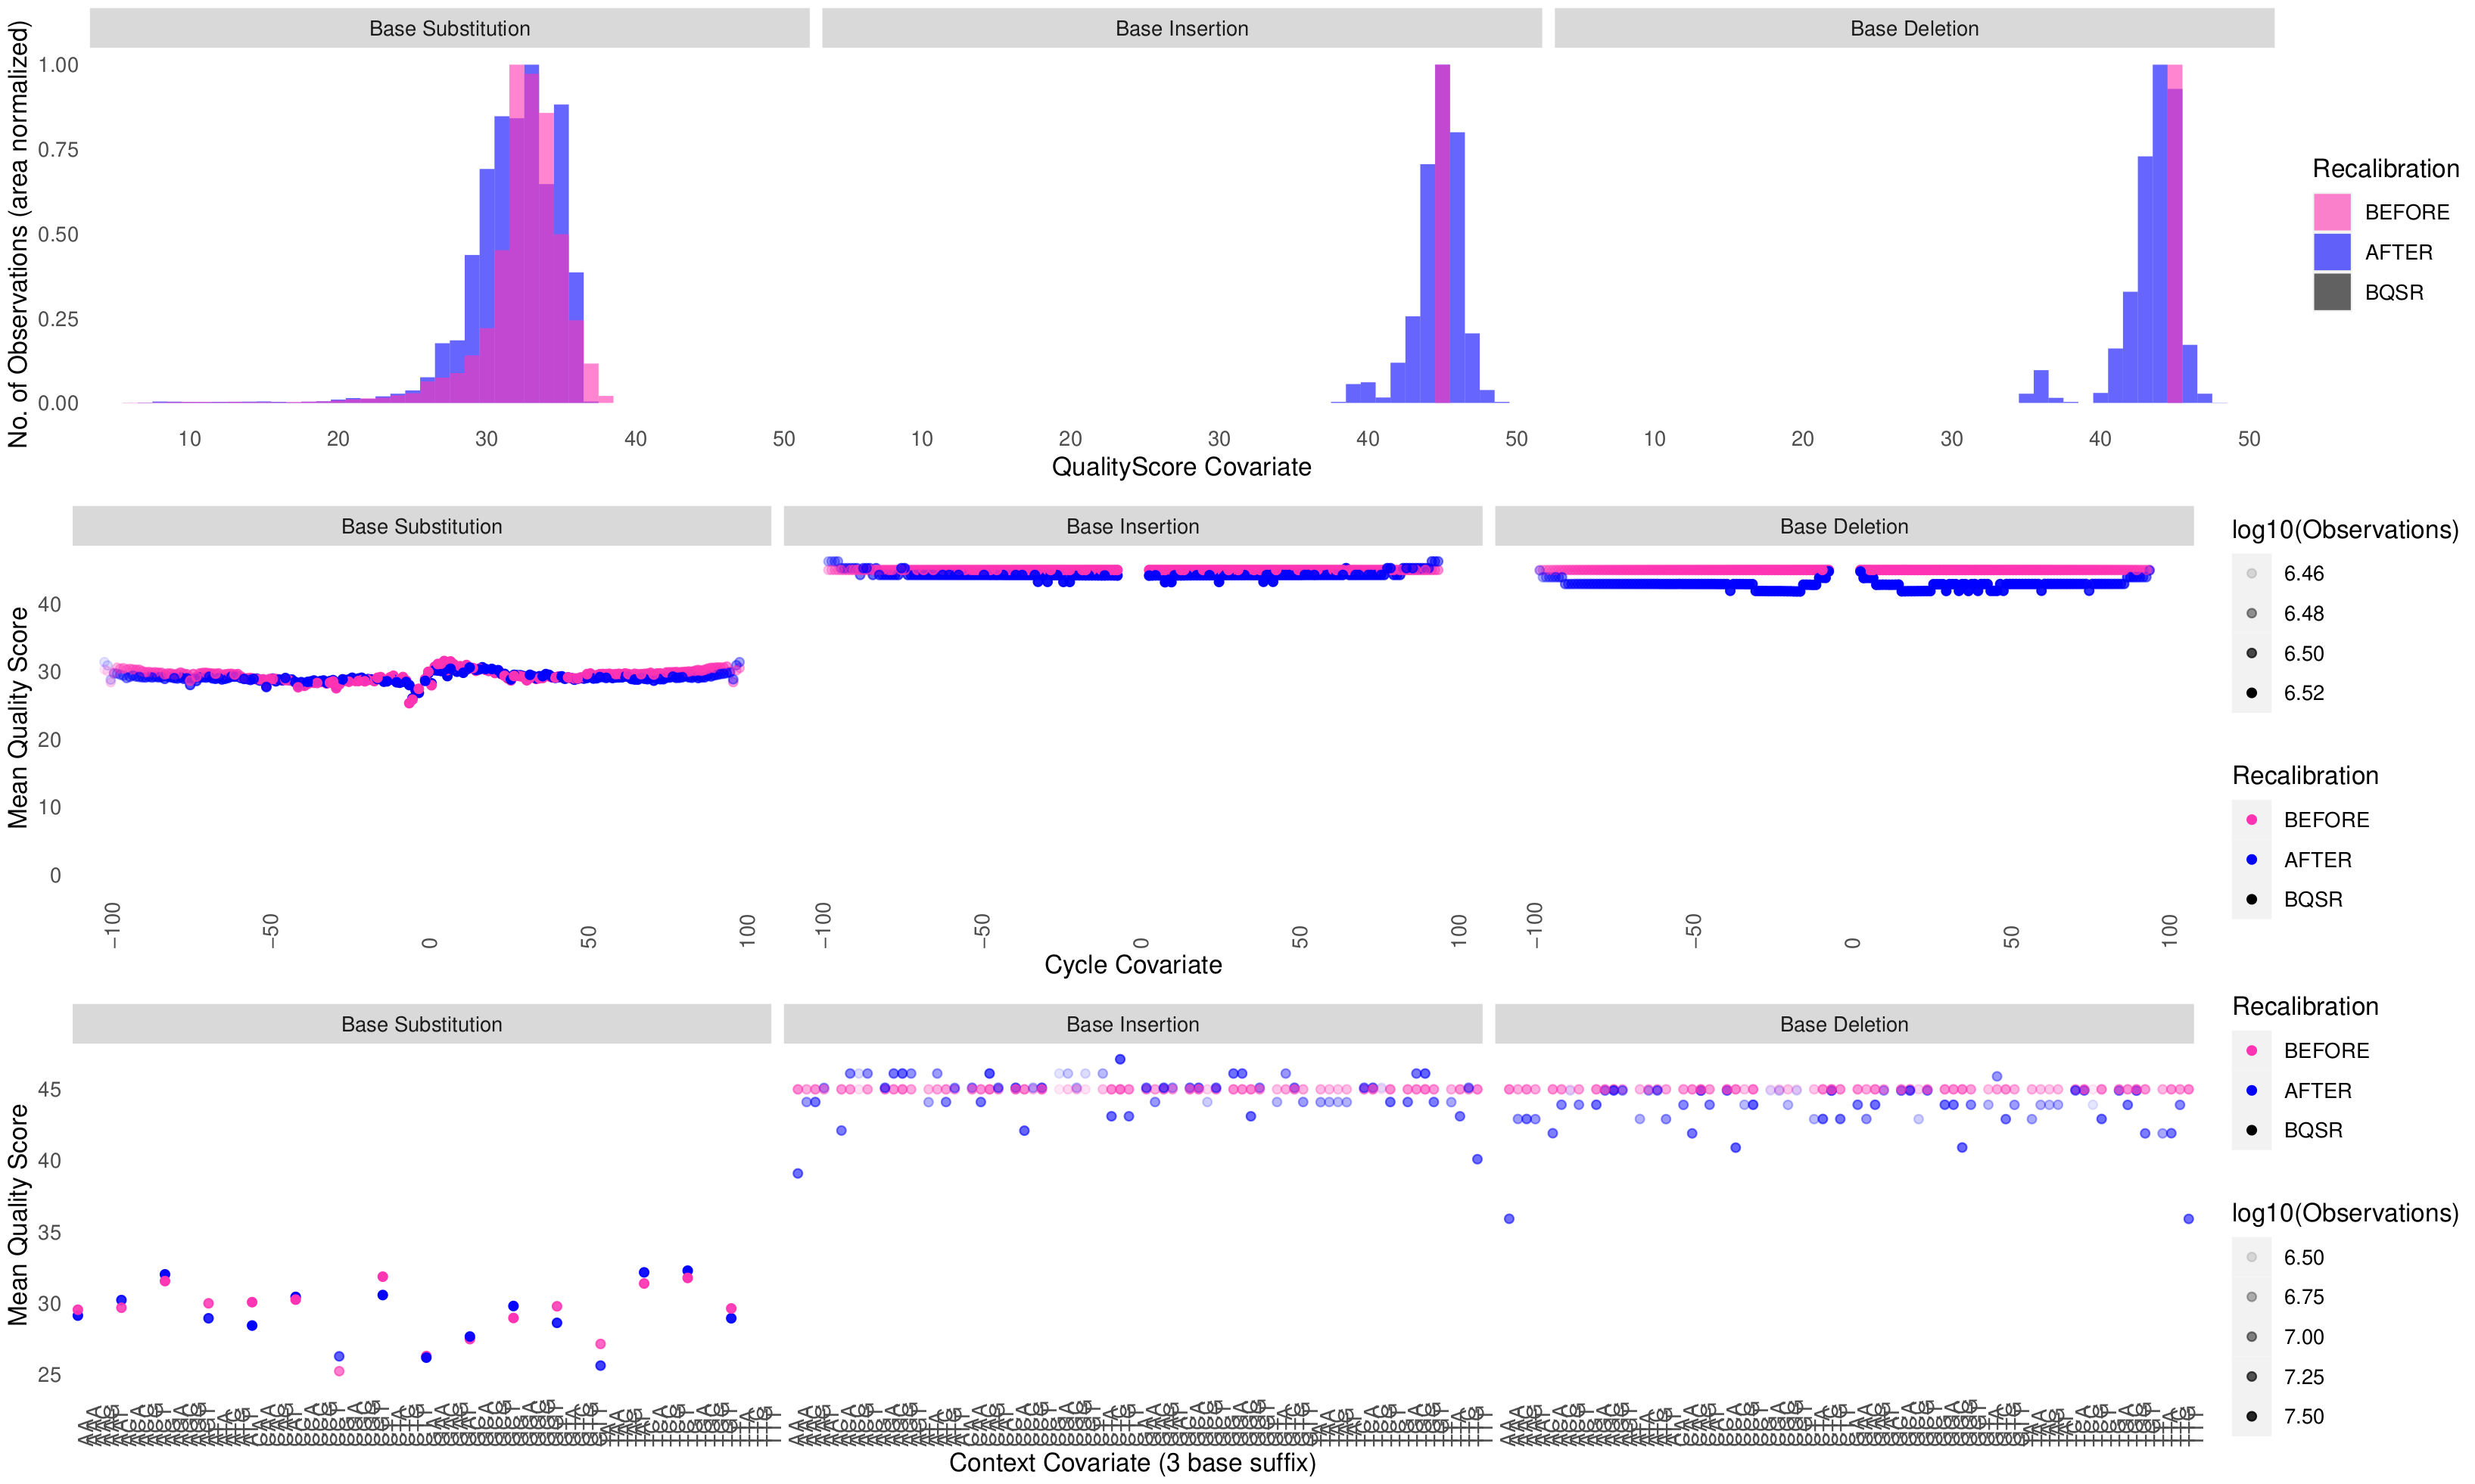
\includegraphics[width=\textwidth]{images/recal_tumor_2_setup1.png}
   \caption{\footnotesize{Recalibration tumor sample}}
   \label{recal_tumor_2}
\end{figure}

\begin{figure}[h]
   \centering
   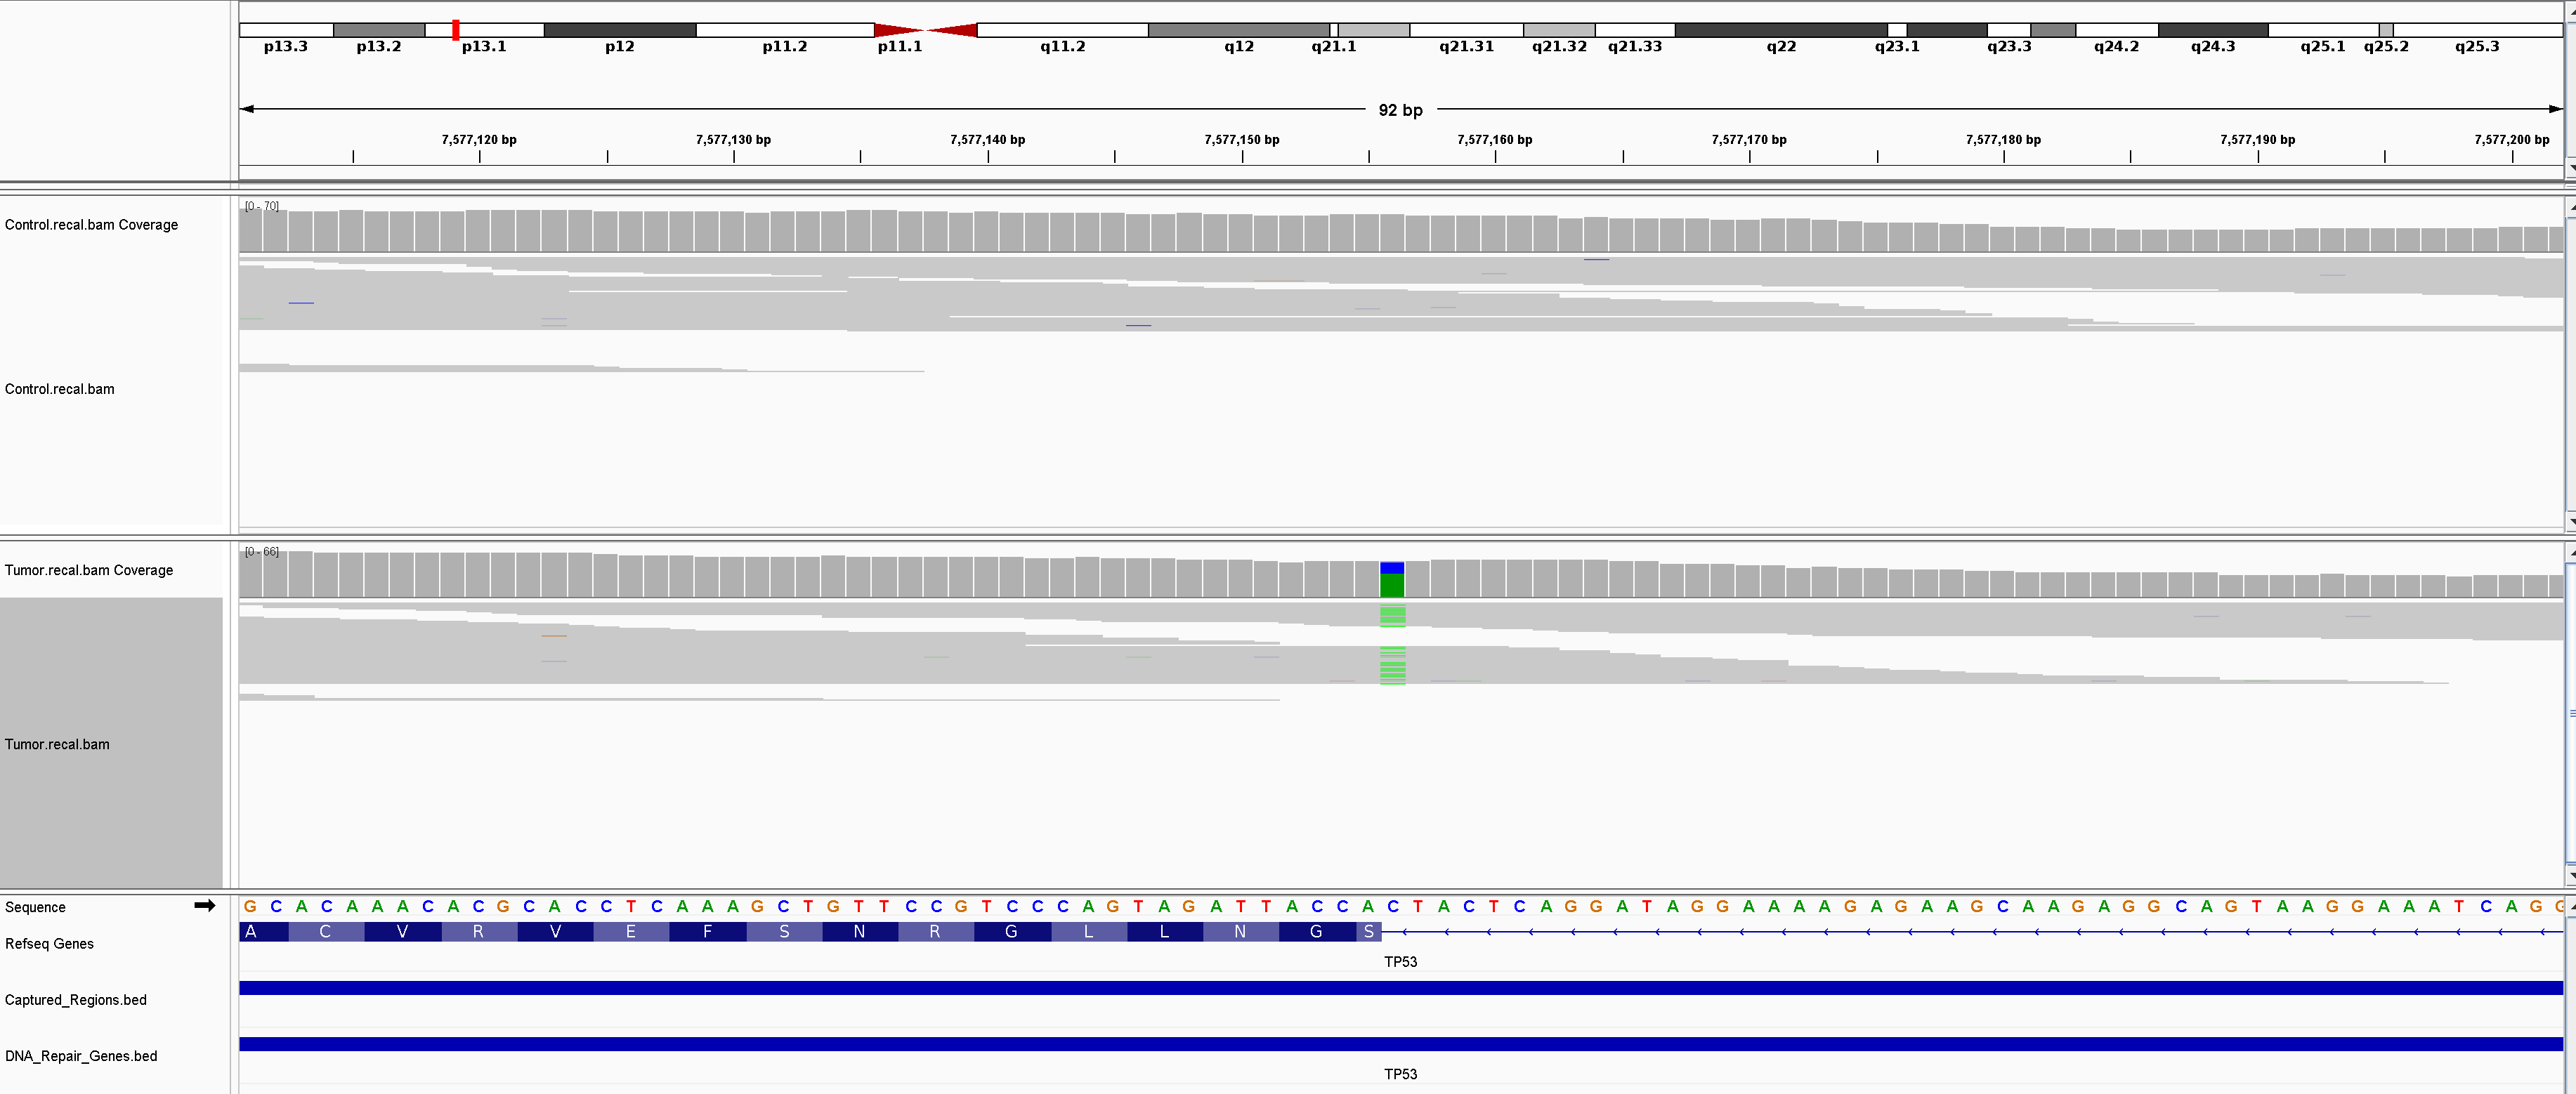
\includegraphics[width=\textwidth]{images/somatic_p53_pm.png}
   \caption{\footnotesize{Somatic point mutation identified with Mutect2 in \emph{TP53} at position chr17:7577156}}
   \label{pm_p53}
\end{figure}

\begin{figure}[h]
   \centering
   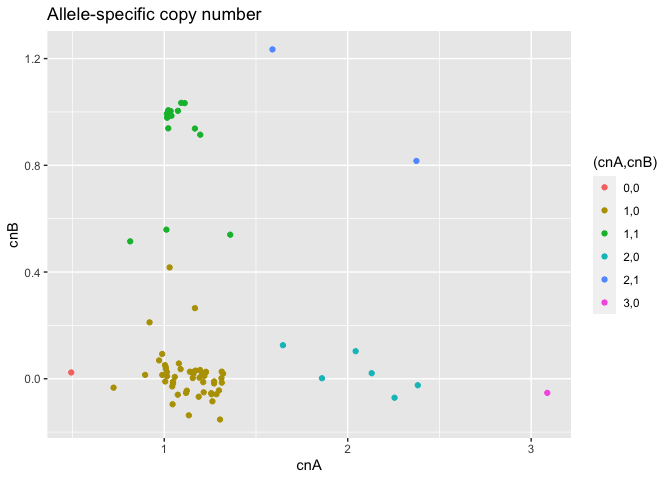
\includegraphics[width=0.5\textwidth]{images/allele-specific-cn.png}
   \caption{\footnotesize{Allele-specific copy-number results obtained with CLONETv2}}
   \label{cn}
\end{figure}


\clearpage

\nocite{Poplin201178}

\printbibliography



\end{document}